\documentclass[twoside]{book}

% Packages required by doxygen
\usepackage{fixltx2e}
\usepackage{calc}
\usepackage{doxygen}
\usepackage[export]{adjustbox} % also loads graphicx
\usepackage{graphicx}
\usepackage[utf8]{inputenc}
\usepackage{makeidx}
\usepackage{multicol}
\usepackage{multirow}
\PassOptionsToPackage{warn}{textcomp}
\usepackage{textcomp}
\usepackage[nointegrals]{wasysym}
\usepackage[table]{xcolor}

% Font selection
\usepackage[T1]{fontenc}
\usepackage[scaled=.90]{helvet}
\usepackage{courier}
\usepackage{amssymb}
\usepackage{sectsty}
\renewcommand{\familydefault}{\sfdefault}
\allsectionsfont{%
  \fontseries{bc}\selectfont%
  \color{darkgray}%
}
\renewcommand{\DoxyLabelFont}{%
  \fontseries{bc}\selectfont%
  \color{darkgray}%
}
\newcommand{\+}{\discretionary{\mbox{\scriptsize$\hookleftarrow$}}{}{}}

% Page & text layout
\usepackage{geometry}
\geometry{%
  a4paper,%
  top=2.5cm,%
  bottom=2.5cm,%
  left=2.5cm,%
  right=2.5cm%
}
\tolerance=750
\hfuzz=15pt
\hbadness=750
\setlength{\emergencystretch}{15pt}
\setlength{\parindent}{0cm}
\setlength{\parskip}{3ex plus 2ex minus 2ex}
\makeatletter
\renewcommand{\paragraph}{%
  \@startsection{paragraph}{4}{0ex}{-1.0ex}{1.0ex}{%
    \normalfont\normalsize\bfseries\SS@parafont%
  }%
}
\renewcommand{\subparagraph}{%
  \@startsection{subparagraph}{5}{0ex}{-1.0ex}{1.0ex}{%
    \normalfont\normalsize\bfseries\SS@subparafont%
  }%
}
\makeatother

% Headers & footers
\usepackage{fancyhdr}
\pagestyle{fancyplain}
\fancyhead[LE]{\fancyplain{}{\bfseries\thepage}}
\fancyhead[CE]{\fancyplain{}{}}
\fancyhead[RE]{\fancyplain{}{\bfseries\leftmark}}
\fancyhead[LO]{\fancyplain{}{\bfseries\rightmark}}
\fancyhead[CO]{\fancyplain{}{}}
\fancyhead[RO]{\fancyplain{}{\bfseries\thepage}}
\fancyfoot[LE]{\fancyplain{}{}}
\fancyfoot[CE]{\fancyplain{}{}}
\fancyfoot[RE]{\fancyplain{}{\bfseries\scriptsize Generated by Doxygen }}
\fancyfoot[LO]{\fancyplain{}{\bfseries\scriptsize Generated by Doxygen }}
\fancyfoot[CO]{\fancyplain{}{}}
\fancyfoot[RO]{\fancyplain{}{}}
\renewcommand{\footrulewidth}{0.4pt}
\renewcommand{\chaptermark}[1]{%
  \markboth{#1}{}%
}
\renewcommand{\sectionmark}[1]{%
  \markright{\thesection\ #1}%
}

% Indices & bibliography
\usepackage{natbib}
\usepackage[titles]{tocloft}
\setcounter{tocdepth}{3}
\setcounter{secnumdepth}{5}
\makeindex

% Custom commands
\newcommand{\clearemptydoublepage}{%
  \newpage{\pagestyle{empty}\cleardoublepage}%
}

\usepackage{caption}
\captionsetup{labelsep=space,justification=centering,font={bf},singlelinecheck=off,skip=4pt,position=top}

%===== C O N T E N T S =====

\begin{document}

% Titlepage & ToC
\pagenumbering{alph}
\begin{titlepage}
\vspace*{7cm}
\begin{center}%
{\Large Firmware B\+R\+D\+Q\+B\+R\+Q\+BC = H\+F\+W2 documentation -\/ qbcontrol main board }\\
\vspace*{1cm}
{\large Generated by Doxygen 1.8.13}\\
\end{center}
\end{titlepage}
\clearemptydoublepage
\pagenumbering{roman}
\tableofcontents
\clearemptydoublepage
\pagenumbering{arabic}

%--- Begin generated contents ---
\chapter{Firmware}
\label{index}This is the firmware of W\+F\+YD. \begin{DoxyVersion}{Version}
1.\+0
\end{DoxyVersion}
This is the firmware of the W\+F\+YD. It can control two motors and a servo motors and read their encoders. Also can read and convert analog measurements connected to the P\+SoC microcontroller. 
\chapter{Data Structure Index}
\section{Data Structures}
Here are the data structures with brief descriptions\+:\begin{DoxyCompactList}
\item\contentsline{section}{\textbf{ st\+\_\+data} }{\pageref{structst__data}}{}
\item\contentsline{section}{\textbf{ st\+\_\+meas} }{\pageref{structst__meas}}{}
\item\contentsline{section}{\textbf{ st\+\_\+mem} }{\pageref{structst__mem}}{}
\item\contentsline{section}{\textbf{ st\+\_\+ref} }{\pageref{structst__ref}}{}
\end{DoxyCompactList}

\chapter{File Index}
\section{File List}
Here is a list of all documented files with brief descriptions\+:\begin{DoxyCompactList}
\item\contentsline{section}{\textbf{ command\+\_\+processing.\+c} \\*Command processing functions }{\pageref{command__processing_8c}}{}
\item\contentsline{section}{\textbf{ command\+\_\+processing.\+h} \\*Command processing functions }{\pageref{command__processing_8h}}{}
\item\contentsline{section}{\textbf{ commands.\+h} \\*Definitions for commands, parameters and packages }{\pageref{commands_8h}}{}
\item\contentsline{section}{{\bfseries device.\+h} }{\pageref{device_8h}}{}
\item\contentsline{section}{\textbf{ globals.\+c} \\*Global variables }{\pageref{globals_8c}}{}
\item\contentsline{section}{\textbf{ globals.\+h} \\*Global definitions and macros are set in this file }{\pageref{globals_8h}}{}
\item\contentsline{section}{\textbf{ interruptions.\+c} \\*Interruption functions are in this file }{\pageref{interruptions_8c}}{}
\item\contentsline{section}{\textbf{ interruptions.\+h} \\*Interruptions header file }{\pageref{interruptions_8h}}{}
\item\contentsline{section}{\textbf{ main.\+c} \\*Firmware main file }{\pageref{main_8c}}{}
\item\contentsline{section}{\textbf{ utils.\+h} \\*Definition of utility functions }{\pageref{utils_8h}}{}
\end{DoxyCompactList}

\chapter{Data Structure Documentation}
\section{st\+\_\+data Struct Reference}
\label{structst__data}\index{st\+\_\+data@{st\+\_\+data}}
\subsection*{Data Fields}
\begin{DoxyCompactItemize}
\item 
\mbox{\label{structst__data_ae690fc5f3d08456a861f43937912613d}} 
uint8 {\bfseries buffer} [128]
\item 
\mbox{\label{structst__data_a3fb0e45fa764ccedd2dd8c0654c2e743}} 
int16 {\bfseries length}
\item 
\mbox{\label{structst__data_a5d76dba8ca72d027d149ffcf8760f2ca}} 
int16 {\bfseries ind}
\item 
\mbox{\label{structst__data_ac24f07ab21d61d7af9cb3a49d102e0ac}} 
uint8 {\bfseries ready}
\end{DoxyCompactItemize}


The documentation for this struct was generated from the following file\+:\begin{DoxyCompactItemize}
\item 
\textbf{ globals.\+h}\end{DoxyCompactItemize}

\section{st\+\_\+meas Struct Reference}
\label{structst__meas}\index{st\+\_\+meas@{st\+\_\+meas}}
\subsection*{Data Fields}
\begin{DoxyCompactItemize}
\item 
\mbox{\label{structst__meas_a3ee4913e7257d25d3e47cbbada9c8546}} 
int32 {\bfseries pos} [N\+U\+M\+\_\+\+O\+F\+\_\+\+S\+E\+N\+S\+O\+RS]
\item 
\mbox{\label{structst__meas_aec90a36a08ebccee4e4a476d2c6e82a5}} 
int16 {\bfseries curr} [N\+U\+M\+\_\+\+O\+F\+\_\+\+M\+O\+T\+O\+RS]
\item 
\mbox{\label{structst__meas_a26b47db1884c475bc42d76a709349f97}} 
int8 {\bfseries rot} [N\+U\+M\+\_\+\+O\+F\+\_\+\+S\+E\+N\+S\+O\+RS]
\item 
\mbox{\label{structst__meas_ad77c8d1a6800fe7da9ebed5c54a1e3b5}} 
int16 {\bfseries vel} [N\+U\+M\+\_\+\+O\+F\+\_\+\+S\+E\+N\+S\+O\+RS]
\item 
\mbox{\label{structst__meas_a3748adf2edf02ab9e3cd7f4fc5b0d2e6}} 
int16 {\bfseries acc} [N\+U\+M\+\_\+\+O\+F\+\_\+\+S\+E\+N\+S\+O\+RS]
\item 
\mbox{\label{structst__meas_ab348be48d334a17631f5e903c9970daa}} 
int16 {\bfseries ir}
\item 
\mbox{\label{structst__meas_a1350f7247a0831ee4668901a6150e2b1}} 
int16 {\bfseries servo}
\item 
\mbox{\label{structst__meas_afe4da6ac27bc16d2e0a965fd3b7c79a9}} 
int16 {\bfseries force}
\item 
\mbox{\label{structst__meas_a50ad0c89371ae2ecde0ec87e03ab13c6}} 
float {\bfseries duty\+\_\+cycle\+\_\+f}
\end{DoxyCompactItemize}


The documentation for this struct was generated from the following file\+:\begin{DoxyCompactItemize}
\item 
\textbf{ globals.\+h}\end{DoxyCompactItemize}

\section{st\+\_\+mem Struct Reference}
\label{structst__mem}\index{st\+\_\+mem@{st\+\_\+mem}}
\subsection*{Data Fields}
\begin{DoxyCompactItemize}
\item 
\mbox{\label{structst__mem_af11e40d15a1361229a78e772af5b3c94}} 
uint8 {\bfseries flag}
\item 
\mbox{\label{structst__mem_a492bfda30c3852a68b2cbfba9531e3d1}} 
uint8 {\bfseries id}
\item 
\mbox{\label{structst__mem_ad1bc394122aa9760c3fc2887a1891cd8}} 
int32 {\bfseries k\+\_\+p}
\item 
\mbox{\label{structst__mem_ad62fb8a39e2de160e14be47e3ff08014}} 
int32 {\bfseries k\+\_\+i}
\item 
\mbox{\label{structst__mem_ab9d15eaa4612dd1c5597e5634cd1d66c}} 
int32 {\bfseries k\+\_\+d}
\item 
\mbox{\label{structst__mem_a96f2aec80e40c1bbe82186a4261ab7ac}} 
int16 {\bfseries current\+\_\+limit}
\item 
\mbox{\label{structst__mem_a63bbebc1db55f43e0571006597a3488b}} 
uint8 {\bfseries activ}
\item 
\mbox{\label{structst__mem_ac2e19d167eac4c8ca9ce97c646e78595}} 
uint8 {\bfseries res} [N\+U\+M\+\_\+\+O\+F\+\_\+\+S\+E\+N\+S\+O\+RS]
\item 
\mbox{\label{structst__mem_ab544f035124be893918bafb611fe88d9}} 
int32 {\bfseries m\+\_\+off} [N\+U\+M\+\_\+\+O\+F\+\_\+\+S\+E\+N\+S\+O\+RS]
\item 
\mbox{\label{structst__mem_aecf0baab567443534c0ded663b746896}} 
float {\bfseries m\+\_\+mult} [N\+U\+M\+\_\+\+O\+F\+\_\+\+S\+E\+N\+S\+O\+RS]
\item 
\mbox{\label{structst__mem_aa2ceebf7546e978c8b0393ce8035532d}} 
uint8 {\bfseries pos\+\_\+lim\+\_\+flag}
\item 
\mbox{\label{structst__mem_a631265c712a620e03d9233634e1819a2}} 
int32 {\bfseries pos\+\_\+lim\+\_\+inf} [N\+U\+M\+\_\+\+O\+F\+\_\+\+M\+O\+T\+O\+RS]
\item 
\mbox{\label{structst__mem_a818808d7c324999701b5aad40a8fabca}} 
int32 {\bfseries pos\+\_\+lim\+\_\+sup} [N\+U\+M\+\_\+\+O\+F\+\_\+\+M\+O\+T\+O\+RS]
\item 
\mbox{\label{structst__mem_aa20cd7437de72c537fd6bb84c158d51e}} 
uint16 {\bfseries max\+\_\+stiffness}
\item 
\mbox{\label{structst__mem_a1a2b3002580421effeca67955a862580}} 
uint8 {\bfseries baud\+\_\+rate}
\item 
\mbox{\label{structst__mem_a1aae70aad54a04c7b41a8d2dcd7aba14}} 
uint8 {\bfseries watchdog\+\_\+period}
\item 
\mbox{\label{structst__mem_a14fe3ed96d232dced2d33efc493a0667}} 
int32 {\bfseries max\+\_\+step\+\_\+neg}
\item 
\mbox{\label{structst__mem_a9be5987152b8c6bb28c1d311bc94e5e3}} 
int32 {\bfseries max\+\_\+step\+\_\+pos}
\item 
\mbox{\label{structst__mem_a60d82b418b3e6aa50300893cfc519a58}} 
int32 {\bfseries thr\+\_\+max\+\_\+force}
\item 
\mbox{\label{structst__mem_ab847275f75384c298dbbe9192b3b76e2}} 
int32 {\bfseries thr\+\_\+max\+\_\+pressure}
\item 
\mbox{\label{structst__mem_a858982429b2aa30b4d460806051b8cce}} 
int32 {\bfseries thr\+\_\+min\+\_\+pressure}
\item 
\mbox{\label{structst__mem_af83e1417974b4fbb30bb2243f200faeb}} 
int32 {\bfseries thr\+\_\+min\+\_\+force}
\item 
\mbox{\label{structst__mem_afa5e5478a19c622ec178dd922e17d5d8}} 
uint8 {\bfseries flag\+\_\+pulse}
\item 
\mbox{\label{structst__mem_adf608da2ecf07896b8ab840a2c66ff9a}} 
double {\bfseries step\+\_\+const}
\item 
\mbox{\label{structst__mem_ac0ec3d2c05fa21e51b7403a8190da3ff}} 
int32 {\bfseries pulse\+\_\+freq}
\item 
\mbox{\label{structst__mem_a59ed30e5aa7ccfd0b5f77c0805ac76f3}} 
uint16 {\bfseries power\+\_\+tension}
\end{DoxyCompactItemize}


The documentation for this struct was generated from the following file\+:\begin{DoxyCompactItemize}
\item 
\textbf{ globals.\+h}\end{DoxyCompactItemize}

\section{st\+\_\+ref Struct Reference}
\label{structst__ref}\index{st\+\_\+ref@{st\+\_\+ref}}
\subsection*{Data Fields}
\begin{DoxyCompactItemize}
\item 
\mbox{\label{structst__ref_a4ac6e991f146f79c274e21a17cfff0a0}} 
int32 {\bfseries pos} [N\+U\+M\+\_\+\+O\+F\+\_\+\+M\+O\+T\+O\+RS]
\item 
\mbox{\label{structst__ref_aea636dc117fd774b0cbfc5e936eac3e5}} 
uint8 {\bfseries onoff}
\end{DoxyCompactItemize}


The documentation for this struct was generated from the following file\+:\begin{DoxyCompactItemize}
\item 
\textbf{ globals.\+h}\end{DoxyCompactItemize}

\chapter{File Documentation}
\section{command\+\_\+processing.\+c File Reference}
\label{command__processing_8c}\index{command\+\_\+processing.\+c@{command\+\_\+processing.\+c}}


Command processing functions.  


{\ttfamily \#include $<$command\+\_\+processing.\+h$>$}\newline
{\ttfamily \#include $<$stdio.\+h$>$}\newline
{\ttfamily \#include $<$interruptions.\+h$>$}\newline
{\ttfamily \#include $<$utils.\+h$>$}\newline
{\ttfamily \#include \char`\"{}commands.\+h\char`\"{}}\newline
Include dependency graph for command\+\_\+processing.\+c\+:
\nopagebreak
\begin{figure}[H]
\begin{center}
\leavevmode
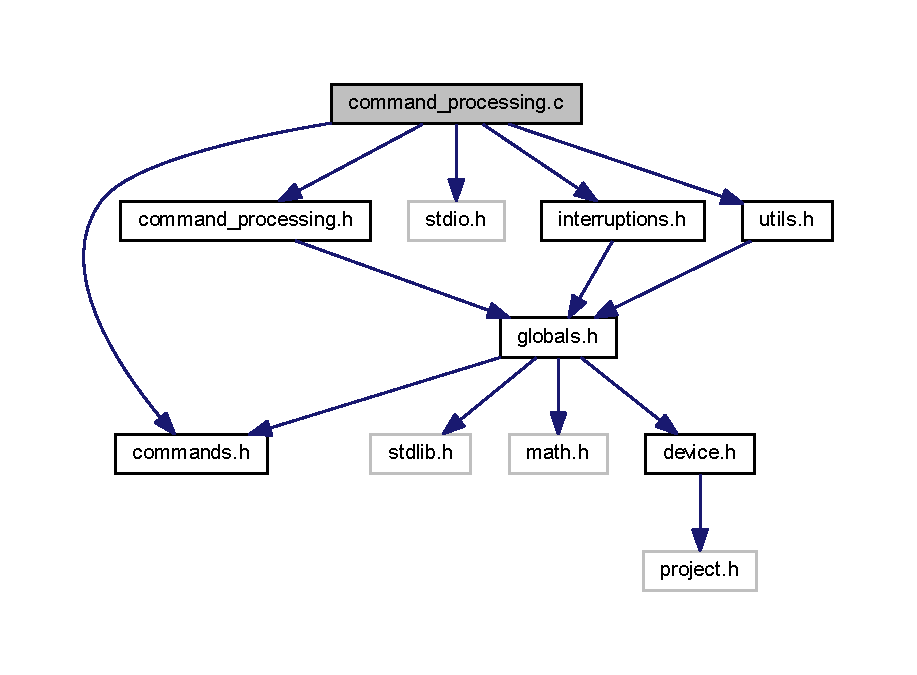
\includegraphics[width=350pt]{command__processing_8c__incl}
\end{center}
\end{figure}
\subsection*{Functions}
\begin{DoxyCompactItemize}
\item 
\mbox{\label{command__processing_8c_a2e5d1711e19837adc3e8f479af3ae509}} 
void {\bfseries comm\+Process} ()
\item 
\mbox{\label{command__processing_8c_a525ccbc7ac3901d938dc352172ee2531}} 
void {\bfseries info\+Get} (uint16 info\+\_\+type)
\item 
\mbox{\label{command__processing_8c_ac8969cb5fdb4916f259075029741e727}} 
void {\bfseries set\+Zeros} ()
\item 
\mbox{\label{command__processing_8c_a5ef086c932682ca5f7549b74ead732aa}} 
void {\bfseries get\+\_\+param\+\_\+list} (uint16 index)
\item 
\mbox{\label{command__processing_8c_abacf855ed80e3052a5bb5b243a0d809e}} 
void {\bfseries info\+Prepare} (unsigned char $\ast$info\+\_\+string)
\item 
\mbox{\label{command__processing_8c_a517f4c61166381d40767fce9011e3c96}} 
void {\bfseries comm\+Write\+\_\+old\+\_\+id} (uint8 $\ast$packet\+\_\+data, uint16 packet\+\_\+lenght, uint8 old\+\_\+id)
\item 
\mbox{\label{command__processing_8c_a1a4919b18b8f9ea21abebd5836a8f35a}} 
void {\bfseries comm\+Write} (uint8 $\ast$packet\+\_\+data, const uint16 packet\+\_\+lenght, uint8 next)
\item 
\mbox{\label{command__processing_8c_af4a42b25376d2efd09096cbbed2fbce4}} 
void {\bfseries send\+Acknowledgment} (const uint8 value)
\item 
uint8 \textbf{ mem\+Store} (int displacement)
\item 
void \textbf{ mem\+Recall} (void)
\item 
uint8 \textbf{ mem\+Restore} (void)
\item 
uint8 \textbf{ mem\+Init} (void)
\item 
void \textbf{ cmd\+\_\+get\+\_\+measurements} ()
\item 
\mbox{\label{command__processing_8c_a20db4694e8caa572ec479f73ce8b3b02}} 
void {\bfseries cmd\+\_\+get\+\_\+inputs} ()
\item 
\mbox{\label{command__processing_8c_aaf613e251c1e14fe4fffe3e9e033f9f7}} 
void {\bfseries cmd\+\_\+get\+\_\+currents} ()
\item 
\mbox{\label{command__processing_8c_a45a90a8455bfdb6a7f0e118da2c6f0a6}} 
void {\bfseries cmd\+\_\+get\+\_\+curr\+\_\+and\+\_\+meas} ()
\item 
\mbox{\label{command__processing_8c_a2d8a4542f55af960a27f875b00aad6a1}} 
void {\bfseries cmd\+\_\+set\+\_\+inputs} ()
\item 
\mbox{\label{command__processing_8c_a212883283bd7a8f32846615271cad8ce}} 
void {\bfseries cmd\+\_\+get\+\_\+velocities} ()
\item 
\mbox{\label{command__processing_8c_a107fc9f2982f9a953bdd82aa07279499}} 
void {\bfseries cmd\+\_\+activate} ()
\item 
\mbox{\label{command__processing_8c_aa94cd9c2e2fbfc5b98e84f67569cfe82}} 
void {\bfseries cmd\+\_\+set\+\_\+watchdog} ()
\item 
\mbox{\label{command__processing_8c_a554d563001517bfbc44400a1e999b393}} 
void {\bfseries cmd\+\_\+get\+\_\+activate} ()
\item 
\mbox{\label{command__processing_8c_a704f8c8cb0f4d75f243fc2b79bc34188}} 
void {\bfseries cmd\+\_\+ping} ()
\item 
\mbox{\label{command__processing_8c_a1a2493bfc2f30171d7e7a3bd5aebab14}} 
void {\bfseries cmd\+\_\+store\+\_\+params} ()
\item 
\mbox{\label{command__processing_8c_aa86bf1f2fa69ab5927f7e4e40eb40581}} 
void {\bfseries cmd\+\_\+set\+\_\+baudrate} ()
\item 
\mbox{\label{command__processing_8c_aa8deb0d217c870fb9523ac35b98303ac}} 
void {\bfseries cmd\+\_\+get\+\_\+ir} ()
\item 
\mbox{\label{command__processing_8c_a9fe051a55635782fd7f6caadcc13a2e8}} 
void {\bfseries cmd\+\_\+get\+\_\+servo} ()
\item 
\mbox{\label{command__processing_8c_a6c4d3e3210b0b6495ccac73a03e0cc38}} 
void {\bfseries cmd\+\_\+get\+\_\+force} ()
\item 
\mbox{\label{command__processing_8c_a43fb73e07e991a54dc51896da7795232}} 
void {\bfseries cmd\+\_\+get\+\_\+duty\+\_\+cy\+\_\+max} ()
\end{DoxyCompactItemize}
\subsection*{Variables}
\begin{DoxyCompactItemize}
\item 
\mbox{\label{command__processing_8c_aba5b9353e6d38cc61eb2bd363df61248}} 
reg8 $\ast$ {\bfseries E\+E\+P\+R\+O\+M\+\_\+\+A\+D\+DR} = (reg8 $\ast$) C\+Y\+D\+E\+V\+\_\+\+E\+E\+\_\+\+B\+A\+SE
\end{DoxyCompactItemize}


\subsection{Detailed Description}
Command processing functions. 

\begin{DoxyDate}{Date}
October 01, 2017 
\end{DoxyDate}
\begin{DoxyAuthor}{Author}
{\itshape Centro \char`\"{}\+E.\+Piaggio\char`\"{}} 
\end{DoxyAuthor}
\begin{DoxyCopyright}{Copyright}
(C) 2012-\/2016 qbrobotics. All rights reserved. 

(C) 2017 Centro \char`\"{}\+E.\+Piaggio\char`\"{}. All rights reserved. 
\end{DoxyCopyright}


\subsection{Function Documentation}
\mbox{\label{command__processing_8c_af5ccd403f1d3e49c97bafd6e7713cff3}} 
\index{command\+\_\+processing.\+c@{command\+\_\+processing.\+c}!cmd\+\_\+get\+\_\+measurements@{cmd\+\_\+get\+\_\+measurements}}
\index{cmd\+\_\+get\+\_\+measurements@{cmd\+\_\+get\+\_\+measurements}!command\+\_\+processing.\+c@{command\+\_\+processing.\+c}}
\subsubsection{cmd\+\_\+get\+\_\+measurements()}
{\footnotesize\ttfamily void cmd\+\_\+get\+\_\+measurements (\begin{DoxyParamCaption}{ }\end{DoxyParamCaption})}

Bunch of functions used on request from U\+A\+RT communication \mbox{\label{command__processing_8c_a48f1d2aa212e255d0a3322e576fc8574}} 
\index{command\+\_\+processing.\+c@{command\+\_\+processing.\+c}!mem\+Init@{mem\+Init}}
\index{mem\+Init@{mem\+Init}!command\+\_\+processing.\+c@{command\+\_\+processing.\+c}}
\subsubsection{mem\+Init()}
{\footnotesize\ttfamily uint8 mem\+Init (\begin{DoxyParamCaption}\item[{void}]{ }\end{DoxyParamCaption})}

This function initialize memory when eeprom is compromised. \mbox{\label{command__processing_8c_a494f1f72ae370f0057e5aa3db73ef6fb}} 
\index{command\+\_\+processing.\+c@{command\+\_\+processing.\+c}!mem\+Recall@{mem\+Recall}}
\index{mem\+Recall@{mem\+Recall}!command\+\_\+processing.\+c@{command\+\_\+processing.\+c}}
\subsubsection{mem\+Recall()}
{\footnotesize\ttfamily void mem\+Recall (\begin{DoxyParamCaption}\item[{void}]{ }\end{DoxyParamCaption})}

This function loads user settings from the eeprom. \mbox{\label{command__processing_8c_af67845c368ea7fefb79a1f0baa12134c}} 
\index{command\+\_\+processing.\+c@{command\+\_\+processing.\+c}!mem\+Restore@{mem\+Restore}}
\index{mem\+Restore@{mem\+Restore}!command\+\_\+processing.\+c@{command\+\_\+processing.\+c}}
\subsubsection{mem\+Restore()}
{\footnotesize\ttfamily uint8 mem\+Restore (\begin{DoxyParamCaption}\item[{void}]{ }\end{DoxyParamCaption})}

This function loads default settings from the eeprom. \mbox{\label{command__processing_8c_a81e6b73c0ee52661736a97c08bdb262b}} 
\index{command\+\_\+processing.\+c@{command\+\_\+processing.\+c}!mem\+Store@{mem\+Store}}
\index{mem\+Store@{mem\+Store}!command\+\_\+processing.\+c@{command\+\_\+processing.\+c}}
\subsubsection{mem\+Store()}
{\footnotesize\ttfamily uint8 mem\+Store (\begin{DoxyParamCaption}\item[{int}]{displacement }\end{DoxyParamCaption})}

This function stores current memory settings on the eeprom with the specified displacement 
\section{command\+\_\+processing.\+h File Reference}
\label{command__processing_8h}\index{command\+\_\+processing.\+h@{command\+\_\+processing.\+h}}


Command processing functions.  


{\ttfamily \#include $<$globals.\+h$>$}\newline
Include dependency graph for command\+\_\+processing.\+h\+:
\nopagebreak
\begin{figure}[H]
\begin{center}
\leavevmode
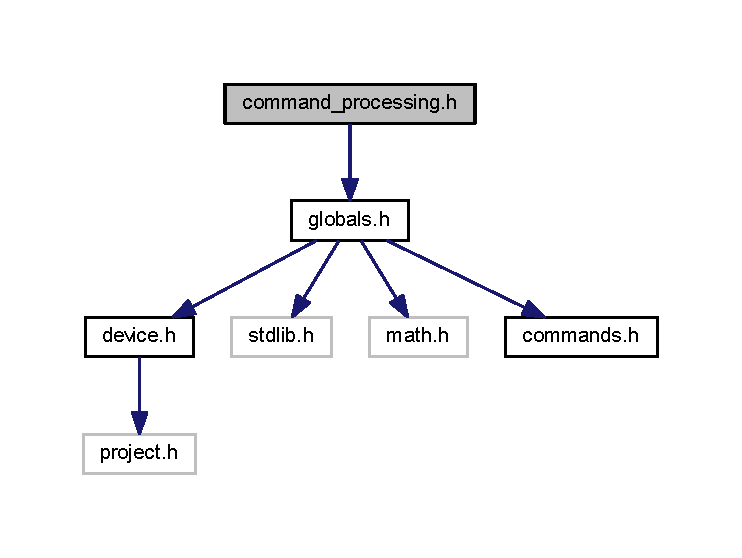
\includegraphics[width=350pt]{command__processing_8h__incl}
\end{center}
\end{figure}
This graph shows which files directly or indirectly include this file\+:
\nopagebreak
\begin{figure}[H]
\begin{center}
\leavevmode
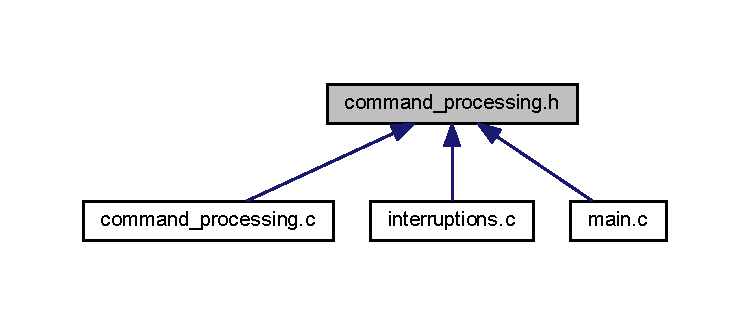
\includegraphics[width=350pt]{command__processing_8h__dep__incl}
\end{center}
\end{figure}
\subsection*{Functions}
\begin{DoxyCompactItemize}
\item 
\mbox{\label{command__processing_8h_abb781ac00e0752ce772a75f7b5d1a5b7}} 
void {\bfseries set\+Zeros} (void)
\item 
\mbox{\label{command__processing_8h_a5ef086c932682ca5f7549b74ead732aa}} 
void {\bfseries get\+\_\+param\+\_\+list} (uint16 index)
\item 
\mbox{\label{command__processing_8h_a6fda7bc0be24d261f9cb09e77616b1be}} 
void {\bfseries info\+Prepare} (unsigned char $\ast$)
\item 
\mbox{\label{command__processing_8h_a813734e69ea461791f84bddee422013f}} 
void {\bfseries info\+Get} (uint16)
\item 
\mbox{\label{command__processing_8h_a2e5d1711e19837adc3e8f479af3ae509}} 
void {\bfseries comm\+Process} ()
\item 
\mbox{\label{command__processing_8h_af59b7a35df04af1df698749a771890eb}} 
void {\bfseries comm\+Write} (uint8 $\ast$, const uint16, uint8)
\item 
\mbox{\label{command__processing_8h_af454a3663070706183ebf8f1ba784343}} 
void {\bfseries comm\+Write\+\_\+old\+\_\+id} (uint8 $\ast$, const uint16, uint8)
\item 
uint8 \textbf{ mem\+Store} (int)
\item 
\mbox{\label{command__processing_8h_afe5c87f9df9bb965976b5d40c4159f1f}} 
void {\bfseries send\+Acknowledgment} (const uint8)
\item 
void \textbf{ mem\+Recall} (void)
\item 
uint8 \textbf{ mem\+Restore} (void)
\item 
uint8 \textbf{ mem\+Init} (void)
\item 
void \textbf{ cmd\+\_\+get\+\_\+measurements} ()
\item 
\mbox{\label{command__processing_8h_a20db4694e8caa572ec479f73ce8b3b02}} 
void {\bfseries cmd\+\_\+get\+\_\+inputs} ()
\item 
\mbox{\label{command__processing_8h_aaf613e251c1e14fe4fffe3e9e033f9f7}} 
void {\bfseries cmd\+\_\+get\+\_\+currents} ()
\item 
\mbox{\label{command__processing_8h_a45a90a8455bfdb6a7f0e118da2c6f0a6}} 
void {\bfseries cmd\+\_\+get\+\_\+curr\+\_\+and\+\_\+meas} ()
\item 
\mbox{\label{command__processing_8h_a2d8a4542f55af960a27f875b00aad6a1}} 
void {\bfseries cmd\+\_\+set\+\_\+inputs} ()
\item 
\mbox{\label{command__processing_8h_a212883283bd7a8f32846615271cad8ce}} 
void {\bfseries cmd\+\_\+get\+\_\+velocities} ()
\item 
\mbox{\label{command__processing_8h_a107fc9f2982f9a953bdd82aa07279499}} 
void {\bfseries cmd\+\_\+activate} ()
\item 
\mbox{\label{command__processing_8h_aa94cd9c2e2fbfc5b98e84f67569cfe82}} 
void {\bfseries cmd\+\_\+set\+\_\+watchdog} ()
\item 
\mbox{\label{command__processing_8h_a554d563001517bfbc44400a1e999b393}} 
void {\bfseries cmd\+\_\+get\+\_\+activate} ()
\item 
\mbox{\label{command__processing_8h_a704f8c8cb0f4d75f243fc2b79bc34188}} 
void {\bfseries cmd\+\_\+ping} ()
\item 
\mbox{\label{command__processing_8h_a1a2493bfc2f30171d7e7a3bd5aebab14}} 
void {\bfseries cmd\+\_\+store\+\_\+params} ()
\item 
\mbox{\label{command__processing_8h_aa86bf1f2fa69ab5927f7e4e40eb40581}} 
void {\bfseries cmd\+\_\+set\+\_\+baudrate} ()
\item 
\mbox{\label{command__processing_8h_aa8deb0d217c870fb9523ac35b98303ac}} 
void {\bfseries cmd\+\_\+get\+\_\+ir} ()
\item 
\mbox{\label{command__processing_8h_a9fe051a55635782fd7f6caadcc13a2e8}} 
void {\bfseries cmd\+\_\+get\+\_\+servo} ()
\item 
\mbox{\label{command__processing_8h_a6c4d3e3210b0b6495ccac73a03e0cc38}} 
void {\bfseries cmd\+\_\+get\+\_\+force} ()
\item 
\mbox{\label{command__processing_8h_a43fb73e07e991a54dc51896da7795232}} 
void {\bfseries cmd\+\_\+get\+\_\+duty\+\_\+cy\+\_\+max} ()
\end{DoxyCompactItemize}


\subsection{Detailed Description}
Command processing functions. 

\begin{DoxyDate}{Date}
October 01, 2017 
\end{DoxyDate}
\begin{DoxyAuthor}{Author}
{\itshape Centro \char`\"{}\+E.\+Piaggio\char`\"{}} 
\end{DoxyAuthor}
\begin{DoxyCopyright}{Copyright}
(C) 2012-\/2016 qbrobotics. All rights reserved. 

(C) 2017 Centro \char`\"{}\+E.\+Piaggio\char`\"{}. All rights reserved. 
\end{DoxyCopyright}


\subsection{Function Documentation}
\mbox{\label{command__processing_8h_af5ccd403f1d3e49c97bafd6e7713cff3}} 
\index{command\+\_\+processing.\+h@{command\+\_\+processing.\+h}!cmd\+\_\+get\+\_\+measurements@{cmd\+\_\+get\+\_\+measurements}}
\index{cmd\+\_\+get\+\_\+measurements@{cmd\+\_\+get\+\_\+measurements}!command\+\_\+processing.\+h@{command\+\_\+processing.\+h}}
\subsubsection{cmd\+\_\+get\+\_\+measurements()}
{\footnotesize\ttfamily void cmd\+\_\+get\+\_\+measurements (\begin{DoxyParamCaption}{ }\end{DoxyParamCaption})}

Bunch of functions used on request from U\+A\+RT communication \mbox{\label{command__processing_8h_a48f1d2aa212e255d0a3322e576fc8574}} 
\index{command\+\_\+processing.\+h@{command\+\_\+processing.\+h}!mem\+Init@{mem\+Init}}
\index{mem\+Init@{mem\+Init}!command\+\_\+processing.\+h@{command\+\_\+processing.\+h}}
\subsubsection{mem\+Init()}
{\footnotesize\ttfamily uint8 mem\+Init (\begin{DoxyParamCaption}\item[{void}]{ }\end{DoxyParamCaption})}

This function initialize memory when eeprom is compromised. \mbox{\label{command__processing_8h_a494f1f72ae370f0057e5aa3db73ef6fb}} 
\index{command\+\_\+processing.\+h@{command\+\_\+processing.\+h}!mem\+Recall@{mem\+Recall}}
\index{mem\+Recall@{mem\+Recall}!command\+\_\+processing.\+h@{command\+\_\+processing.\+h}}
\subsubsection{mem\+Recall()}
{\footnotesize\ttfamily void mem\+Recall (\begin{DoxyParamCaption}\item[{void}]{ }\end{DoxyParamCaption})}

This function loads user settings from the eeprom. \mbox{\label{command__processing_8h_af67845c368ea7fefb79a1f0baa12134c}} 
\index{command\+\_\+processing.\+h@{command\+\_\+processing.\+h}!mem\+Restore@{mem\+Restore}}
\index{mem\+Restore@{mem\+Restore}!command\+\_\+processing.\+h@{command\+\_\+processing.\+h}}
\subsubsection{mem\+Restore()}
{\footnotesize\ttfamily uint8 mem\+Restore (\begin{DoxyParamCaption}\item[{void}]{ }\end{DoxyParamCaption})}

This function loads default settings from the eeprom. \mbox{\label{command__processing_8h_ad37da1fb5c1ccf35a9a53595b8bab54c}} 
\index{command\+\_\+processing.\+h@{command\+\_\+processing.\+h}!mem\+Store@{mem\+Store}}
\index{mem\+Store@{mem\+Store}!command\+\_\+processing.\+h@{command\+\_\+processing.\+h}}
\subsubsection{mem\+Store()}
{\footnotesize\ttfamily uint8 mem\+Store (\begin{DoxyParamCaption}\item[{int}]{displacement }\end{DoxyParamCaption})}

This function stores current memory settings on the eeprom with the specified displacement 
\section{commands.\+h File Reference}
\label{commands_8h}\index{commands.\+h@{commands.\+h}}


Definitions for board commands, parameters and packages.  


This graph shows which files directly or indirectly include this file\+:
\nopagebreak
\begin{figure}[H]
\begin{center}
\leavevmode
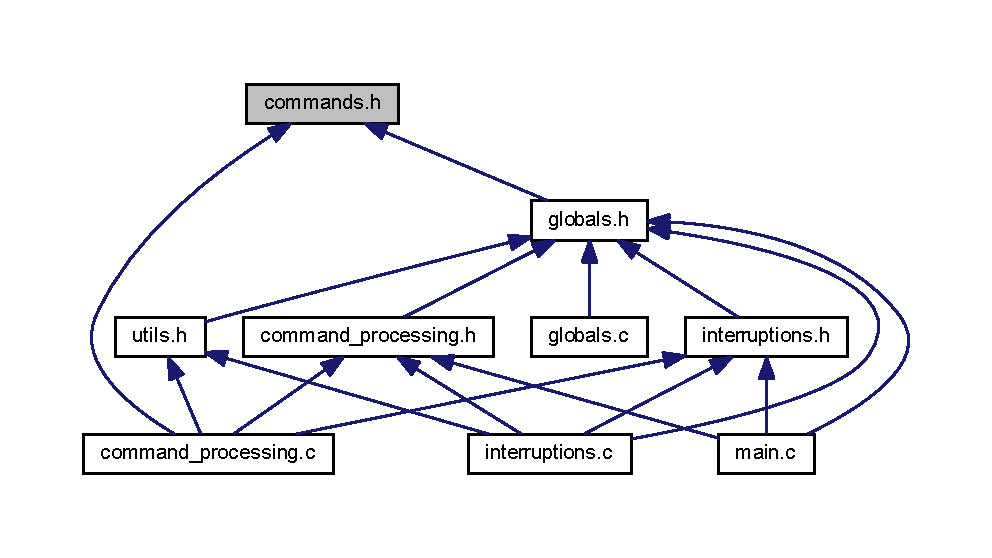
\includegraphics[width=350pt]{commands_8h__dep__incl}
\end{center}
\end{figure}
\subsection*{Macros}
\begin{DoxyCompactItemize}
\item 
\mbox{\label{commands_8h_ad97188edfdd667de971027b35330fa41}} 
\#define {\bfseries A\+P\+I\+\_\+\+V\+E\+R\+S\+I\+ON}~\char`\"{}v6.\+1.\+0\char`\"{}
\end{DoxyCompactItemize}
\begin{Indent}\textbf{ QB Move Information Strings}\par
\begin{DoxyCompactItemize}
\item 
\mbox{\label{commands_8h_a2ba44fc5b8a316bd307d0baa9ab629ef}} 
\#define \textbf{ I\+N\+F\+O\+\_\+\+A\+LL}~0
\begin{DoxyCompactList}\small\item\em All system information. \end{DoxyCompactList}\end{DoxyCompactItemize}
\end{Indent}
\subsection*{Enumerations}
\begin{Indent}\textbf{ qb\+Move and qb\+Hand Commands}\par
\begin{DoxyCompactItemize}
\item 
enum \textbf{ qbmove\+\_\+command} \{ \newline
\textbf{ C\+M\+D\+\_\+\+P\+I\+NG} = 0, 
\textbf{ C\+M\+D\+\_\+\+S\+E\+T\+\_\+\+Z\+E\+R\+OS} = 1, 
\textbf{ C\+M\+D\+\_\+\+S\+T\+O\+R\+E\+\_\+\+P\+A\+R\+A\+MS} = 3, 
\textbf{ C\+M\+D\+\_\+\+S\+T\+O\+R\+E\+\_\+\+D\+E\+F\+A\+U\+L\+T\+\_\+\+P\+A\+R\+A\+MS} = 4, 
\newline
\textbf{ C\+M\+D\+\_\+\+R\+E\+S\+T\+O\+R\+E\+\_\+\+P\+A\+R\+A\+MS} = 5, 
\textbf{ C\+M\+D\+\_\+\+G\+E\+T\+\_\+\+I\+N\+FO} = 6, 
\textbf{ C\+M\+D\+\_\+\+S\+E\+T\+\_\+\+V\+A\+L\+UE} = 7, 
\textbf{ C\+M\+D\+\_\+\+G\+E\+T\+\_\+\+V\+A\+L\+UE} = 8, 
\newline
\textbf{ C\+M\+D\+\_\+\+B\+O\+O\+T\+L\+O\+A\+D\+ER} = 9, 
\textbf{ C\+M\+D\+\_\+\+I\+N\+I\+T\+\_\+\+M\+EM} = 10, 
\textbf{ C\+M\+D\+\_\+\+C\+A\+L\+I\+B\+R\+A\+TE} = 11, 
\textbf{ C\+M\+D\+\_\+\+G\+E\+T\+\_\+\+P\+A\+R\+A\+M\+\_\+\+L\+I\+ST} = 12, 
\newline
\textbf{ C\+M\+D\+\_\+\+H\+A\+N\+D\+\_\+\+C\+A\+L\+I\+B\+R\+A\+TE} = 13, 
\textbf{ C\+M\+D\+\_\+\+A\+C\+T\+I\+V\+A\+TE} = 128, 
\textbf{ C\+M\+D\+\_\+\+G\+E\+T\+\_\+\+A\+C\+T\+I\+V\+A\+TE} = 129, 
\textbf{ C\+M\+D\+\_\+\+S\+E\+T\+\_\+\+I\+N\+P\+U\+TS} = 130, 
\newline
\textbf{ C\+M\+D\+\_\+\+G\+E\+T\+\_\+\+I\+N\+P\+U\+TS} = 131, 
\textbf{ C\+M\+D\+\_\+\+G\+E\+T\+\_\+\+M\+E\+A\+S\+U\+R\+E\+M\+E\+N\+TS} = 132, 
\textbf{ C\+M\+D\+\_\+\+G\+E\+T\+\_\+\+C\+U\+R\+R\+E\+N\+TS} = 133, 
\textbf{ C\+M\+D\+\_\+\+G\+E\+T\+\_\+\+C\+U\+R\+R\+\_\+\+A\+N\+D\+\_\+\+M\+E\+AS} = 134, 
\newline
\textbf{ C\+M\+D\+\_\+\+S\+E\+T\+\_\+\+P\+O\+S\+\_\+\+S\+T\+I\+FF} = 135, 
\textbf{ C\+M\+D\+\_\+\+G\+E\+T\+\_\+\+E\+MG} = 136, 
\textbf{ C\+M\+D\+\_\+\+G\+E\+T\+\_\+\+V\+E\+L\+O\+C\+I\+T\+I\+ES} = 137, 
\textbf{ C\+M\+D\+\_\+\+G\+E\+T\+\_\+\+C\+O\+U\+N\+T\+E\+RS} = 138, 
\newline
\textbf{ C\+M\+D\+\_\+\+G\+E\+T\+\_\+\+A\+C\+C\+EL} = 139, 
\textbf{ C\+M\+D\+\_\+\+G\+E\+T\+\_\+\+C\+U\+R\+R\+\_\+\+D\+I\+FF} = 140, 
\textbf{ C\+M\+D\+\_\+\+S\+E\+T\+\_\+\+C\+U\+R\+R\+\_\+\+D\+I\+FF} = 141, 
\textbf{ C\+M\+D\+\_\+\+S\+E\+T\+\_\+\+C\+U\+F\+F\+\_\+\+I\+N\+P\+U\+TS} = 142, 
\newline
\textbf{ C\+M\+D\+\_\+\+S\+E\+T\+\_\+\+W\+A\+T\+C\+H\+D\+OG} = 143, 
\textbf{ C\+M\+D\+\_\+\+S\+E\+T\+\_\+\+B\+A\+U\+D\+R\+A\+TE} = 144, 
\textbf{ C\+M\+D\+\_\+\+E\+X\+T\+\_\+\+D\+R\+I\+VE} = 145, 
\textbf{ C\+M\+D\+\_\+\+G\+E\+T\+\_\+\+J\+O\+Y\+S\+T\+I\+CK} = 146
 \}
\end{DoxyCompactItemize}
\end{Indent}
\subsection*{qb\+Move and qb\+Hand Parameters}
\begin{DoxyCompactItemize}
\item 
\mbox{\label{commands_8h_ae3302107827a773be3200e459e7b24da}} 
\#define {\bfseries P\+A\+R\+A\+M\+\_\+\+B\+Y\+T\+E\+\_\+\+S\+L\+OT}~50
\item 
\mbox{\label{commands_8h_a3bab5133f6aa363d84307b39e17b0d74}} 
\#define {\bfseries P\+A\+R\+A\+M\+\_\+\+M\+E\+N\+U\+\_\+\+S\+L\+OT}~150
\item 
enum \textbf{ qbmove\+\_\+parameter} \{ \newline
\textbf{ P\+A\+R\+A\+M\+\_\+\+ID} = 0, 
\textbf{ P\+A\+R\+A\+M\+\_\+\+P\+I\+D\+\_\+\+C\+O\+N\+T\+R\+OL} = 1, 
\textbf{ P\+A\+R\+A\+M\+\_\+\+S\+T\+A\+R\+T\+U\+P\+\_\+\+A\+C\+T\+I\+V\+A\+T\+I\+ON} = 2, 
\textbf{ P\+A\+R\+A\+M\+\_\+\+I\+N\+P\+U\+T\+\_\+\+M\+O\+DE} = 3, 
\newline
\textbf{ P\+A\+R\+A\+M\+\_\+\+C\+O\+N\+T\+R\+O\+L\+\_\+\+M\+O\+DE} = 4, 
\textbf{ P\+A\+R\+A\+M\+\_\+\+M\+E\+A\+S\+U\+R\+E\+M\+E\+N\+T\+\_\+\+O\+F\+F\+S\+ET} = 5, 
\textbf{ P\+A\+R\+A\+M\+\_\+\+M\+E\+A\+S\+U\+R\+E\+M\+E\+N\+T\+\_\+\+M\+U\+L\+T\+I\+P\+L\+I\+ER} = 6, 
\textbf{ P\+A\+R\+A\+M\+\_\+\+P\+O\+S\+\_\+\+L\+I\+M\+I\+T\+\_\+\+F\+L\+AG} = 7, 
\newline
\textbf{ P\+A\+R\+A\+M\+\_\+\+P\+O\+S\+\_\+\+L\+I\+M\+IT} = 8, 
\textbf{ P\+A\+R\+A\+M\+\_\+\+M\+A\+X\+\_\+\+S\+T\+E\+P\+\_\+\+P\+OS} = 9, 
\textbf{ P\+A\+R\+A\+M\+\_\+\+M\+A\+X\+\_\+\+S\+T\+E\+P\+\_\+\+N\+EG} = 10, 
\textbf{ P\+A\+R\+A\+M\+\_\+\+P\+O\+S\+\_\+\+R\+E\+S\+O\+L\+U\+T\+I\+ON} = 11, 
\newline
\textbf{ P\+A\+R\+A\+M\+\_\+\+C\+U\+R\+R\+E\+N\+T\+\_\+\+L\+I\+M\+IT} = 12, 
\textbf{ P\+A\+R\+A\+M\+\_\+\+E\+M\+G\+\_\+\+C\+A\+L\+I\+B\+\_\+\+F\+L\+AG} = 13, 
\textbf{ P\+A\+R\+A\+M\+\_\+\+E\+M\+G\+\_\+\+T\+H\+R\+E\+S\+H\+O\+LD} = 14, 
\textbf{ P\+A\+R\+A\+M\+\_\+\+E\+M\+G\+\_\+\+M\+A\+X\+\_\+\+V\+A\+L\+UE} = 15, 
\newline
\textbf{ P\+A\+R\+A\+M\+\_\+\+E\+M\+G\+\_\+\+S\+P\+E\+ED} = 16, 
\textbf{ P\+A\+R\+A\+M\+\_\+\+P\+I\+D\+\_\+\+C\+U\+R\+R\+\_\+\+C\+O\+N\+T\+R\+OL} = 18, 
\textbf{ P\+A\+R\+A\+M\+\_\+\+D\+O\+U\+B\+L\+E\+\_\+\+E\+N\+C\+\_\+\+O\+N\+\_\+\+O\+FF} = 19, 
\textbf{ P\+A\+R\+A\+M\+\_\+\+M\+O\+T\+\_\+\+H\+A\+N\+D\+L\+E\+\_\+\+R\+A\+T\+IO} = 20, 
\newline
\textbf{ P\+A\+R\+A\+M\+\_\+\+M\+O\+T\+O\+R\+\_\+\+S\+U\+P\+P\+LY} = 21, 
\textbf{ P\+A\+R\+A\+M\+\_\+\+C\+U\+R\+R\+E\+N\+T\+\_\+\+L\+O\+O\+K\+UP} = 23, 
\textbf{ P\+A\+R\+A\+M\+\_\+\+D\+L\+\_\+\+P\+O\+S\+\_\+\+P\+ID} = 24, 
\textbf{ P\+A\+R\+A\+M\+\_\+\+D\+L\+\_\+\+C\+U\+R\+R\+\_\+\+P\+ID} = 25
 \}
\item 
\mbox{\label{commands_8h_ad18f2ef316ee226b52882af5758c39e8}} 
enum {\bfseries qbmove\+\_\+resolution} \{ \newline
{\bfseries R\+E\+S\+O\+L\+U\+T\+I\+O\+N\+\_\+360} = 0, 
{\bfseries R\+E\+S\+O\+L\+U\+T\+I\+O\+N\+\_\+720} = 1, 
{\bfseries R\+E\+S\+O\+L\+U\+T\+I\+O\+N\+\_\+1440} = 2, 
{\bfseries R\+E\+S\+O\+L\+U\+T\+I\+O\+N\+\_\+2880} = 3, 
\newline
{\bfseries R\+E\+S\+O\+L\+U\+T\+I\+O\+N\+\_\+5760} = 4, 
{\bfseries R\+E\+S\+O\+L\+U\+T\+I\+O\+N\+\_\+11520} = 5, 
{\bfseries R\+E\+S\+O\+L\+U\+T\+I\+O\+N\+\_\+23040} = 6, 
{\bfseries R\+E\+S\+O\+L\+U\+T\+I\+O\+N\+\_\+46080} = 7, 
\newline
{\bfseries R\+E\+S\+O\+L\+U\+T\+I\+O\+N\+\_\+92160} = 8
 \}
\item 
enum \textbf{ qbmove\+\_\+input\+\_\+mode} \{ \newline
\textbf{ I\+N\+P\+U\+T\+\_\+\+M\+O\+D\+E\+\_\+\+E\+X\+T\+E\+R\+N\+AL} = 0, 
\textbf{ I\+N\+P\+U\+T\+\_\+\+M\+O\+D\+E\+\_\+\+E\+N\+C\+O\+D\+E\+R3} = 1, 
\textbf{ I\+N\+P\+U\+T\+\_\+\+M\+O\+D\+E\+\_\+\+E\+M\+G\+\_\+\+P\+R\+O\+P\+O\+R\+T\+I\+O\+N\+AL} = 2, 
\textbf{ I\+N\+P\+U\+T\+\_\+\+M\+O\+D\+E\+\_\+\+E\+M\+G\+\_\+\+I\+N\+T\+E\+G\+R\+AL} = 3, 
\newline
\textbf{ I\+N\+P\+U\+T\+\_\+\+M\+O\+D\+E\+\_\+\+E\+M\+G\+\_\+\+F\+C\+FS} = 4, 
\textbf{ I\+N\+P\+U\+T\+\_\+\+M\+O\+D\+E\+\_\+\+E\+M\+G\+\_\+\+F\+C\+F\+S\+\_\+\+A\+DV} = 5
 \}
\item 
enum \textbf{ qbmove\+\_\+control\+\_\+mode} \{ \newline
\textbf{ C\+O\+N\+T\+R\+O\+L\+\_\+\+A\+N\+G\+LE} = 0, 
\textbf{ C\+O\+N\+T\+R\+O\+L\+\_\+\+P\+WM} = 1, 
\textbf{ C\+O\+N\+T\+R\+O\+L\+\_\+\+C\+U\+R\+R\+E\+NT} = 2, 
\textbf{ C\+U\+R\+R\+\_\+\+A\+N\+D\+\_\+\+P\+O\+S\+\_\+\+C\+O\+N\+T\+R\+OL} = 3, 
\newline
\textbf{ D\+E\+F\+L\+E\+C\+T\+I\+O\+N\+\_\+\+C\+O\+N\+T\+R\+OL} = 4, 
\textbf{ D\+E\+F\+L\+\_\+\+C\+U\+R\+R\+E\+N\+T\+\_\+\+C\+O\+N\+T\+R\+OL} = 5
 \}
\item 
\mbox{\label{commands_8h_a17c218160a8b2c5f25db27616793d564}} 
enum {\bfseries motor\+\_\+supply\+\_\+tipe} \{ {\bfseries M\+A\+X\+O\+N\+\_\+24V} = 0, 
{\bfseries M\+A\+X\+O\+N\+\_\+12V} = 1
 \}
\item 
\mbox{\label{commands_8h_a0eae1c82d20671c5d0b9b82b10070f1b}} 
enum {\bfseries acknowledgment\+\_\+values} \{ {\bfseries A\+C\+K\+\_\+\+E\+R\+R\+OR} = 0, 
{\bfseries A\+C\+K\+\_\+\+OK} = 1
 \}
\item 
\mbox{\label{commands_8h_aee7544e5fa6e2843ecdc3609602e56aa}} 
enum {\bfseries data\+\_\+types} \{ \newline
{\bfseries T\+Y\+P\+E\+\_\+\+F\+L\+AG} = 0, 
{\bfseries T\+Y\+P\+E\+\_\+\+I\+N\+T8} = 1, 
{\bfseries T\+Y\+P\+E\+\_\+\+U\+I\+N\+T8} = 2, 
{\bfseries T\+Y\+P\+E\+\_\+\+I\+N\+T16} = 3, 
\newline
{\bfseries T\+Y\+P\+E\+\_\+\+U\+I\+N\+T16} = 4, 
{\bfseries T\+Y\+P\+E\+\_\+\+I\+N\+T32} = 5, 
{\bfseries T\+Y\+P\+E\+\_\+\+U\+I\+N\+T32} = 6, 
{\bfseries T\+Y\+P\+E\+\_\+\+F\+L\+O\+AT} = 7, 
\newline
{\bfseries T\+Y\+P\+E\+\_\+\+D\+O\+U\+B\+LE} = 8
 \}
\end{DoxyCompactItemize}


\subsection{Detailed Description}
Definitions for board commands, parameters and packages. 

\begin{DoxyAuthor}{Author}
{\itshape Centro \char`\"{}\+E.\+Piaggio\char`\"{}} 
\end{DoxyAuthor}
\begin{DoxyCopyright}{Copyright}
(C) 2012-\/2016 qbrobotics. All rights reserved. 

(C) 2017 Centro \char`\"{}\+E.\+Piaggio\char`\"{}. All rights reserved.
\end{DoxyCopyright}
This file is included in the board firmware, in its libraries and applications. It contains all definitions that are necessary for the contruction of communication packages.

It includes definitions for all of the device commands, parameters and also the size of answer packages. 

\subsection{Enumeration Type Documentation}
\mbox{\label{commands_8h_abf0494aabdc65d654a54044eddc9210b}} 
\index{commands.\+h@{commands.\+h}!qbmove\+\_\+command@{qbmove\+\_\+command}}
\index{qbmove\+\_\+command@{qbmove\+\_\+command}!commands.\+h@{commands.\+h}}
\subsubsection{qbmove\+\_\+command}
{\footnotesize\ttfamily enum \textbf{ qbmove\+\_\+command}}

\begin{DoxyEnumFields}{Enumerator}
\raisebox{\heightof{T}}[0pt][0pt]{\index{C\+M\+D\+\_\+\+P\+I\+NG@{C\+M\+D\+\_\+\+P\+I\+NG}!commands.\+h@{commands.\+h}}\index{commands.\+h@{commands.\+h}!C\+M\+D\+\_\+\+P\+I\+NG@{C\+M\+D\+\_\+\+P\+I\+NG}}}\mbox{\label{commands_8h_abf0494aabdc65d654a54044eddc9210ba1c0aa24c3612e77ea1a5ca1b82388da0}} 
C\+M\+D\+\_\+\+P\+I\+NG&Asks for a ping message. \\
\hline

\raisebox{\heightof{T}}[0pt][0pt]{\index{C\+M\+D\+\_\+\+S\+E\+T\+\_\+\+Z\+E\+R\+OS@{C\+M\+D\+\_\+\+S\+E\+T\+\_\+\+Z\+E\+R\+OS}!commands.\+h@{commands.\+h}}\index{commands.\+h@{commands.\+h}!C\+M\+D\+\_\+\+S\+E\+T\+\_\+\+Z\+E\+R\+OS@{C\+M\+D\+\_\+\+S\+E\+T\+\_\+\+Z\+E\+R\+OS}}}\mbox{\label{commands_8h_abf0494aabdc65d654a54044eddc9210ba2d92e89157e03fe63bfebf8125c3a0d7}} 
C\+M\+D\+\_\+\+S\+E\+T\+\_\+\+Z\+E\+R\+OS&Command for setting the encoders zero position. \\
\hline

\raisebox{\heightof{T}}[0pt][0pt]{\index{C\+M\+D\+\_\+\+S\+T\+O\+R\+E\+\_\+\+P\+A\+R\+A\+MS@{C\+M\+D\+\_\+\+S\+T\+O\+R\+E\+\_\+\+P\+A\+R\+A\+MS}!commands.\+h@{commands.\+h}}\index{commands.\+h@{commands.\+h}!C\+M\+D\+\_\+\+S\+T\+O\+R\+E\+\_\+\+P\+A\+R\+A\+MS@{C\+M\+D\+\_\+\+S\+T\+O\+R\+E\+\_\+\+P\+A\+R\+A\+MS}}}\mbox{\label{commands_8h_abf0494aabdc65d654a54044eddc9210bac7d1170961179d8dc5ec1b4aeb4f3116}} 
C\+M\+D\+\_\+\+S\+T\+O\+R\+E\+\_\+\+P\+A\+R\+A\+MS&Stores all parameters in memory and loads them \\
\hline

\raisebox{\heightof{T}}[0pt][0pt]{\index{C\+M\+D\+\_\+\+S\+T\+O\+R\+E\+\_\+\+D\+E\+F\+A\+U\+L\+T\+\_\+\+P\+A\+R\+A\+MS@{C\+M\+D\+\_\+\+S\+T\+O\+R\+E\+\_\+\+D\+E\+F\+A\+U\+L\+T\+\_\+\+P\+A\+R\+A\+MS}!commands.\+h@{commands.\+h}}\index{commands.\+h@{commands.\+h}!C\+M\+D\+\_\+\+S\+T\+O\+R\+E\+\_\+\+D\+E\+F\+A\+U\+L\+T\+\_\+\+P\+A\+R\+A\+MS@{C\+M\+D\+\_\+\+S\+T\+O\+R\+E\+\_\+\+D\+E\+F\+A\+U\+L\+T\+\_\+\+P\+A\+R\+A\+MS}}}\mbox{\label{commands_8h_abf0494aabdc65d654a54044eddc9210ba17d9c730cd01059737de14b9f062e44c}} 
C\+M\+D\+\_\+\+S\+T\+O\+R\+E\+\_\+\+D\+E\+F\+A\+U\+L\+T\+\_\+\+P\+A\+R\+A\+MS&Store current parameters as factory parameters. \\
\hline

\raisebox{\heightof{T}}[0pt][0pt]{\index{C\+M\+D\+\_\+\+R\+E\+S\+T\+O\+R\+E\+\_\+\+P\+A\+R\+A\+MS@{C\+M\+D\+\_\+\+R\+E\+S\+T\+O\+R\+E\+\_\+\+P\+A\+R\+A\+MS}!commands.\+h@{commands.\+h}}\index{commands.\+h@{commands.\+h}!C\+M\+D\+\_\+\+R\+E\+S\+T\+O\+R\+E\+\_\+\+P\+A\+R\+A\+MS@{C\+M\+D\+\_\+\+R\+E\+S\+T\+O\+R\+E\+\_\+\+P\+A\+R\+A\+MS}}}\mbox{\label{commands_8h_abf0494aabdc65d654a54044eddc9210ba7f13c143f54c74572776ffae219d33d7}} 
C\+M\+D\+\_\+\+R\+E\+S\+T\+O\+R\+E\+\_\+\+P\+A\+R\+A\+MS&Restore default factory parameters. \\
\hline

\raisebox{\heightof{T}}[0pt][0pt]{\index{C\+M\+D\+\_\+\+G\+E\+T\+\_\+\+I\+N\+FO@{C\+M\+D\+\_\+\+G\+E\+T\+\_\+\+I\+N\+FO}!commands.\+h@{commands.\+h}}\index{commands.\+h@{commands.\+h}!C\+M\+D\+\_\+\+G\+E\+T\+\_\+\+I\+N\+FO@{C\+M\+D\+\_\+\+G\+E\+T\+\_\+\+I\+N\+FO}}}\mbox{\label{commands_8h_abf0494aabdc65d654a54044eddc9210ba4681b714888632a2d8ad0a2140e4ba7f}} 
C\+M\+D\+\_\+\+G\+E\+T\+\_\+\+I\+N\+FO&Asks for a string of information about. \\
\hline

\raisebox{\heightof{T}}[0pt][0pt]{\index{C\+M\+D\+\_\+\+S\+E\+T\+\_\+\+V\+A\+L\+UE@{C\+M\+D\+\_\+\+S\+E\+T\+\_\+\+V\+A\+L\+UE}!commands.\+h@{commands.\+h}}\index{commands.\+h@{commands.\+h}!C\+M\+D\+\_\+\+S\+E\+T\+\_\+\+V\+A\+L\+UE@{C\+M\+D\+\_\+\+S\+E\+T\+\_\+\+V\+A\+L\+UE}}}\mbox{\label{commands_8h_abf0494aabdc65d654a54044eddc9210bac3ca8989b510cb78baff4425a0d47a67}} 
C\+M\+D\+\_\+\+S\+E\+T\+\_\+\+V\+A\+L\+UE&Not Used. \\
\hline

\raisebox{\heightof{T}}[0pt][0pt]{\index{C\+M\+D\+\_\+\+G\+E\+T\+\_\+\+V\+A\+L\+UE@{C\+M\+D\+\_\+\+G\+E\+T\+\_\+\+V\+A\+L\+UE}!commands.\+h@{commands.\+h}}\index{commands.\+h@{commands.\+h}!C\+M\+D\+\_\+\+G\+E\+T\+\_\+\+V\+A\+L\+UE@{C\+M\+D\+\_\+\+G\+E\+T\+\_\+\+V\+A\+L\+UE}}}\mbox{\label{commands_8h_abf0494aabdc65d654a54044eddc9210bac9a592ed746a114c7bfc0bd9d094263c}} 
C\+M\+D\+\_\+\+G\+E\+T\+\_\+\+V\+A\+L\+UE&Not Used. \\
\hline

\raisebox{\heightof{T}}[0pt][0pt]{\index{C\+M\+D\+\_\+\+B\+O\+O\+T\+L\+O\+A\+D\+ER@{C\+M\+D\+\_\+\+B\+O\+O\+T\+L\+O\+A\+D\+ER}!commands.\+h@{commands.\+h}}\index{commands.\+h@{commands.\+h}!C\+M\+D\+\_\+\+B\+O\+O\+T\+L\+O\+A\+D\+ER@{C\+M\+D\+\_\+\+B\+O\+O\+T\+L\+O\+A\+D\+ER}}}\mbox{\label{commands_8h_abf0494aabdc65d654a54044eddc9210bac72c6075e3464ea5abbe0c0d6e11559e}} 
C\+M\+D\+\_\+\+B\+O\+O\+T\+L\+O\+A\+D\+ER&Sets the bootloader modality to update the firmware \\
\hline

\raisebox{\heightof{T}}[0pt][0pt]{\index{C\+M\+D\+\_\+\+I\+N\+I\+T\+\_\+\+M\+EM@{C\+M\+D\+\_\+\+I\+N\+I\+T\+\_\+\+M\+EM}!commands.\+h@{commands.\+h}}\index{commands.\+h@{commands.\+h}!C\+M\+D\+\_\+\+I\+N\+I\+T\+\_\+\+M\+EM@{C\+M\+D\+\_\+\+I\+N\+I\+T\+\_\+\+M\+EM}}}\mbox{\label{commands_8h_abf0494aabdc65d654a54044eddc9210ba7bd24a7ad88af9a4e7c398a9ecb08ed4}} 
C\+M\+D\+\_\+\+I\+N\+I\+T\+\_\+\+M\+EM&Initialize the memory with the defalut values. \\
\hline

\raisebox{\heightof{T}}[0pt][0pt]{\index{C\+M\+D\+\_\+\+C\+A\+L\+I\+B\+R\+A\+TE@{C\+M\+D\+\_\+\+C\+A\+L\+I\+B\+R\+A\+TE}!commands.\+h@{commands.\+h}}\index{commands.\+h@{commands.\+h}!C\+M\+D\+\_\+\+C\+A\+L\+I\+B\+R\+A\+TE@{C\+M\+D\+\_\+\+C\+A\+L\+I\+B\+R\+A\+TE}}}\mbox{\label{commands_8h_abf0494aabdc65d654a54044eddc9210ba238830aded332d3bd5cbbb4ea2cb6ce7}} 
C\+M\+D\+\_\+\+C\+A\+L\+I\+B\+R\+A\+TE&Starts the stiffness calibration of the qb\+Move. \\
\hline

\raisebox{\heightof{T}}[0pt][0pt]{\index{C\+M\+D\+\_\+\+G\+E\+T\+\_\+\+P\+A\+R\+A\+M\+\_\+\+L\+I\+ST@{C\+M\+D\+\_\+\+G\+E\+T\+\_\+\+P\+A\+R\+A\+M\+\_\+\+L\+I\+ST}!commands.\+h@{commands.\+h}}\index{commands.\+h@{commands.\+h}!C\+M\+D\+\_\+\+G\+E\+T\+\_\+\+P\+A\+R\+A\+M\+\_\+\+L\+I\+ST@{C\+M\+D\+\_\+\+G\+E\+T\+\_\+\+P\+A\+R\+A\+M\+\_\+\+L\+I\+ST}}}\mbox{\label{commands_8h_abf0494aabdc65d654a54044eddc9210ba3e92a6e4c288be3abb6f3cfadf261e78}} 
C\+M\+D\+\_\+\+G\+E\+T\+\_\+\+P\+A\+R\+A\+M\+\_\+\+L\+I\+ST&Command to get the parameters list or to set a defined value chosen by the use \\
\hline

\raisebox{\heightof{T}}[0pt][0pt]{\index{C\+M\+D\+\_\+\+H\+A\+N\+D\+\_\+\+C\+A\+L\+I\+B\+R\+A\+TE@{C\+M\+D\+\_\+\+H\+A\+N\+D\+\_\+\+C\+A\+L\+I\+B\+R\+A\+TE}!commands.\+h@{commands.\+h}}\index{commands.\+h@{commands.\+h}!C\+M\+D\+\_\+\+H\+A\+N\+D\+\_\+\+C\+A\+L\+I\+B\+R\+A\+TE@{C\+M\+D\+\_\+\+H\+A\+N\+D\+\_\+\+C\+A\+L\+I\+B\+R\+A\+TE}}}\mbox{\label{commands_8h_abf0494aabdc65d654a54044eddc9210ba76be5a50e0ac4a9f944d0d6382f06e92}} 
C\+M\+D\+\_\+\+H\+A\+N\+D\+\_\+\+C\+A\+L\+I\+B\+R\+A\+TE&Starts a series of opening and closures of the hand. \\
\hline

\raisebox{\heightof{T}}[0pt][0pt]{\index{C\+M\+D\+\_\+\+A\+C\+T\+I\+V\+A\+TE@{C\+M\+D\+\_\+\+A\+C\+T\+I\+V\+A\+TE}!commands.\+h@{commands.\+h}}\index{commands.\+h@{commands.\+h}!C\+M\+D\+\_\+\+A\+C\+T\+I\+V\+A\+TE@{C\+M\+D\+\_\+\+A\+C\+T\+I\+V\+A\+TE}}}\mbox{\label{commands_8h_abf0494aabdc65d654a54044eddc9210ba341cc0e29a584b4c75a7502529920a7f}} 
C\+M\+D\+\_\+\+A\+C\+T\+I\+V\+A\+TE&Command for activating/deactivating the device \\
\hline

\raisebox{\heightof{T}}[0pt][0pt]{\index{C\+M\+D\+\_\+\+G\+E\+T\+\_\+\+A\+C\+T\+I\+V\+A\+TE@{C\+M\+D\+\_\+\+G\+E\+T\+\_\+\+A\+C\+T\+I\+V\+A\+TE}!commands.\+h@{commands.\+h}}\index{commands.\+h@{commands.\+h}!C\+M\+D\+\_\+\+G\+E\+T\+\_\+\+A\+C\+T\+I\+V\+A\+TE@{C\+M\+D\+\_\+\+G\+E\+T\+\_\+\+A\+C\+T\+I\+V\+A\+TE}}}\mbox{\label{commands_8h_abf0494aabdc65d654a54044eddc9210bac56c7ee3592b79204a8f209460ca6531}} 
C\+M\+D\+\_\+\+G\+E\+T\+\_\+\+A\+C\+T\+I\+V\+A\+TE&Command for getting device activation state \\
\hline

\raisebox{\heightof{T}}[0pt][0pt]{\index{C\+M\+D\+\_\+\+S\+E\+T\+\_\+\+I\+N\+P\+U\+TS@{C\+M\+D\+\_\+\+S\+E\+T\+\_\+\+I\+N\+P\+U\+TS}!commands.\+h@{commands.\+h}}\index{commands.\+h@{commands.\+h}!C\+M\+D\+\_\+\+S\+E\+T\+\_\+\+I\+N\+P\+U\+TS@{C\+M\+D\+\_\+\+S\+E\+T\+\_\+\+I\+N\+P\+U\+TS}}}\mbox{\label{commands_8h_abf0494aabdc65d654a54044eddc9210bac271d0c424b55b263c47f451b3685d65}} 
C\+M\+D\+\_\+\+S\+E\+T\+\_\+\+I\+N\+P\+U\+TS&Command for setting reference inputs. \\
\hline

\raisebox{\heightof{T}}[0pt][0pt]{\index{C\+M\+D\+\_\+\+G\+E\+T\+\_\+\+I\+N\+P\+U\+TS@{C\+M\+D\+\_\+\+G\+E\+T\+\_\+\+I\+N\+P\+U\+TS}!commands.\+h@{commands.\+h}}\index{commands.\+h@{commands.\+h}!C\+M\+D\+\_\+\+G\+E\+T\+\_\+\+I\+N\+P\+U\+TS@{C\+M\+D\+\_\+\+G\+E\+T\+\_\+\+I\+N\+P\+U\+TS}}}\mbox{\label{commands_8h_abf0494aabdc65d654a54044eddc9210ba7e1020474f9835468c3cfbcce610f7df}} 
C\+M\+D\+\_\+\+G\+E\+T\+\_\+\+I\+N\+P\+U\+TS&Command for getting reference inputs. \\
\hline

\raisebox{\heightof{T}}[0pt][0pt]{\index{C\+M\+D\+\_\+\+G\+E\+T\+\_\+\+M\+E\+A\+S\+U\+R\+E\+M\+E\+N\+TS@{C\+M\+D\+\_\+\+G\+E\+T\+\_\+\+M\+E\+A\+S\+U\+R\+E\+M\+E\+N\+TS}!commands.\+h@{commands.\+h}}\index{commands.\+h@{commands.\+h}!C\+M\+D\+\_\+\+G\+E\+T\+\_\+\+M\+E\+A\+S\+U\+R\+E\+M\+E\+N\+TS@{C\+M\+D\+\_\+\+G\+E\+T\+\_\+\+M\+E\+A\+S\+U\+R\+E\+M\+E\+N\+TS}}}\mbox{\label{commands_8h_abf0494aabdc65d654a54044eddc9210bae71f36974018d7c926d1023127ba5018}} 
C\+M\+D\+\_\+\+G\+E\+T\+\_\+\+M\+E\+A\+S\+U\+R\+E\+M\+E\+N\+TS&Command for asking device\textquotesingle{}s position measurements \\
\hline

\raisebox{\heightof{T}}[0pt][0pt]{\index{C\+M\+D\+\_\+\+G\+E\+T\+\_\+\+C\+U\+R\+R\+E\+N\+TS@{C\+M\+D\+\_\+\+G\+E\+T\+\_\+\+C\+U\+R\+R\+E\+N\+TS}!commands.\+h@{commands.\+h}}\index{commands.\+h@{commands.\+h}!C\+M\+D\+\_\+\+G\+E\+T\+\_\+\+C\+U\+R\+R\+E\+N\+TS@{C\+M\+D\+\_\+\+G\+E\+T\+\_\+\+C\+U\+R\+R\+E\+N\+TS}}}\mbox{\label{commands_8h_abf0494aabdc65d654a54044eddc9210ba7cec1501d2f9057540987c1f9f3eaf2d}} 
C\+M\+D\+\_\+\+G\+E\+T\+\_\+\+C\+U\+R\+R\+E\+N\+TS&Command for asking device\textquotesingle{}s current measurements \\
\hline

\raisebox{\heightof{T}}[0pt][0pt]{\index{C\+M\+D\+\_\+\+G\+E\+T\+\_\+\+C\+U\+R\+R\+\_\+\+A\+N\+D\+\_\+\+M\+E\+AS@{C\+M\+D\+\_\+\+G\+E\+T\+\_\+\+C\+U\+R\+R\+\_\+\+A\+N\+D\+\_\+\+M\+E\+AS}!commands.\+h@{commands.\+h}}\index{commands.\+h@{commands.\+h}!C\+M\+D\+\_\+\+G\+E\+T\+\_\+\+C\+U\+R\+R\+\_\+\+A\+N\+D\+\_\+\+M\+E\+AS@{C\+M\+D\+\_\+\+G\+E\+T\+\_\+\+C\+U\+R\+R\+\_\+\+A\+N\+D\+\_\+\+M\+E\+AS}}}\mbox{\label{commands_8h_abf0494aabdc65d654a54044eddc9210ba00e1e21809cce47849f8d237b14c9e17}} 
C\+M\+D\+\_\+\+G\+E\+T\+\_\+\+C\+U\+R\+R\+\_\+\+A\+N\+D\+\_\+\+M\+E\+AS&Command for asking device\textquotesingle{}s measurements and currents \\
\hline

\raisebox{\heightof{T}}[0pt][0pt]{\index{C\+M\+D\+\_\+\+S\+E\+T\+\_\+\+P\+O\+S\+\_\+\+S\+T\+I\+FF@{C\+M\+D\+\_\+\+S\+E\+T\+\_\+\+P\+O\+S\+\_\+\+S\+T\+I\+FF}!commands.\+h@{commands.\+h}}\index{commands.\+h@{commands.\+h}!C\+M\+D\+\_\+\+S\+E\+T\+\_\+\+P\+O\+S\+\_\+\+S\+T\+I\+FF@{C\+M\+D\+\_\+\+S\+E\+T\+\_\+\+P\+O\+S\+\_\+\+S\+T\+I\+FF}}}\mbox{\label{commands_8h_abf0494aabdc65d654a54044eddc9210baa8ff629570855ac5162560c19fcbd374}} 
C\+M\+D\+\_\+\+S\+E\+T\+\_\+\+P\+O\+S\+\_\+\+S\+T\+I\+FF&Not used in the softhand firmware. \\
\hline

\raisebox{\heightof{T}}[0pt][0pt]{\index{C\+M\+D\+\_\+\+G\+E\+T\+\_\+\+E\+MG@{C\+M\+D\+\_\+\+G\+E\+T\+\_\+\+E\+MG}!commands.\+h@{commands.\+h}}\index{commands.\+h@{commands.\+h}!C\+M\+D\+\_\+\+G\+E\+T\+\_\+\+E\+MG@{C\+M\+D\+\_\+\+G\+E\+T\+\_\+\+E\+MG}}}\mbox{\label{commands_8h_abf0494aabdc65d654a54044eddc9210baf64fae1b253023ea4d6307619fb00bd6}} 
C\+M\+D\+\_\+\+G\+E\+T\+\_\+\+E\+MG&Command for asking device\textquotesingle{}s emg sensors measurements \\
\hline

\raisebox{\heightof{T}}[0pt][0pt]{\index{C\+M\+D\+\_\+\+G\+E\+T\+\_\+\+V\+E\+L\+O\+C\+I\+T\+I\+ES@{C\+M\+D\+\_\+\+G\+E\+T\+\_\+\+V\+E\+L\+O\+C\+I\+T\+I\+ES}!commands.\+h@{commands.\+h}}\index{commands.\+h@{commands.\+h}!C\+M\+D\+\_\+\+G\+E\+T\+\_\+\+V\+E\+L\+O\+C\+I\+T\+I\+ES@{C\+M\+D\+\_\+\+G\+E\+T\+\_\+\+V\+E\+L\+O\+C\+I\+T\+I\+ES}}}\mbox{\label{commands_8h_abf0494aabdc65d654a54044eddc9210ba91f95871982459406bcbfa9e84affcf8}} 
C\+M\+D\+\_\+\+G\+E\+T\+\_\+\+V\+E\+L\+O\+C\+I\+T\+I\+ES&Command for asking device\textquotesingle{}s velocity measurements \\
\hline

\raisebox{\heightof{T}}[0pt][0pt]{\index{C\+M\+D\+\_\+\+G\+E\+T\+\_\+\+C\+O\+U\+N\+T\+E\+RS@{C\+M\+D\+\_\+\+G\+E\+T\+\_\+\+C\+O\+U\+N\+T\+E\+RS}!commands.\+h@{commands.\+h}}\index{commands.\+h@{commands.\+h}!C\+M\+D\+\_\+\+G\+E\+T\+\_\+\+C\+O\+U\+N\+T\+E\+RS@{C\+M\+D\+\_\+\+G\+E\+T\+\_\+\+C\+O\+U\+N\+T\+E\+RS}}}\mbox{\label{commands_8h_abf0494aabdc65d654a54044eddc9210ba852a1e9b4cec526ef7b4e550cee73cae}} 
C\+M\+D\+\_\+\+G\+E\+T\+\_\+\+C\+O\+U\+N\+T\+E\+RS&Command for asking device\textquotesingle{}s counters (mostly used for debugging sent commands) \\
\hline

\raisebox{\heightof{T}}[0pt][0pt]{\index{C\+M\+D\+\_\+\+G\+E\+T\+\_\+\+A\+C\+C\+EL@{C\+M\+D\+\_\+\+G\+E\+T\+\_\+\+A\+C\+C\+EL}!commands.\+h@{commands.\+h}}\index{commands.\+h@{commands.\+h}!C\+M\+D\+\_\+\+G\+E\+T\+\_\+\+A\+C\+C\+EL@{C\+M\+D\+\_\+\+G\+E\+T\+\_\+\+A\+C\+C\+EL}}}\mbox{\label{commands_8h_abf0494aabdc65d654a54044eddc9210ba62e954ab85dca16967b1d2b11f099515}} 
C\+M\+D\+\_\+\+G\+E\+T\+\_\+\+A\+C\+C\+EL&Command for asking device\textquotesingle{}s acceleration measurements \\
\hline

\raisebox{\heightof{T}}[0pt][0pt]{\index{C\+M\+D\+\_\+\+G\+E\+T\+\_\+\+C\+U\+R\+R\+\_\+\+D\+I\+FF@{C\+M\+D\+\_\+\+G\+E\+T\+\_\+\+C\+U\+R\+R\+\_\+\+D\+I\+FF}!commands.\+h@{commands.\+h}}\index{commands.\+h@{commands.\+h}!C\+M\+D\+\_\+\+G\+E\+T\+\_\+\+C\+U\+R\+R\+\_\+\+D\+I\+FF@{C\+M\+D\+\_\+\+G\+E\+T\+\_\+\+C\+U\+R\+R\+\_\+\+D\+I\+FF}}}\mbox{\label{commands_8h_abf0494aabdc65d654a54044eddc9210bac1a1e6554eb0603ea5a5f77f604f594c}} 
C\+M\+D\+\_\+\+G\+E\+T\+\_\+\+C\+U\+R\+R\+\_\+\+D\+I\+FF&Command for asking device\textquotesingle{}s current difference between a measured one and an estimated one (Only for Soft\+Hand) \\
\hline

\raisebox{\heightof{T}}[0pt][0pt]{\index{C\+M\+D\+\_\+\+S\+E\+T\+\_\+\+C\+U\+R\+R\+\_\+\+D\+I\+FF@{C\+M\+D\+\_\+\+S\+E\+T\+\_\+\+C\+U\+R\+R\+\_\+\+D\+I\+FF}!commands.\+h@{commands.\+h}}\index{commands.\+h@{commands.\+h}!C\+M\+D\+\_\+\+S\+E\+T\+\_\+\+C\+U\+R\+R\+\_\+\+D\+I\+FF@{C\+M\+D\+\_\+\+S\+E\+T\+\_\+\+C\+U\+R\+R\+\_\+\+D\+I\+FF}}}\mbox{\label{commands_8h_abf0494aabdc65d654a54044eddc9210ba75bb0f4bbebcfa9d066c0d1f41531127}} 
C\+M\+D\+\_\+\+S\+E\+T\+\_\+\+C\+U\+R\+R\+\_\+\+D\+I\+FF&Command used to set current difference modality (Only for Cuff device) \\
\hline

\raisebox{\heightof{T}}[0pt][0pt]{\index{C\+M\+D\+\_\+\+S\+E\+T\+\_\+\+C\+U\+F\+F\+\_\+\+I\+N\+P\+U\+TS@{C\+M\+D\+\_\+\+S\+E\+T\+\_\+\+C\+U\+F\+F\+\_\+\+I\+N\+P\+U\+TS}!commands.\+h@{commands.\+h}}\index{commands.\+h@{commands.\+h}!C\+M\+D\+\_\+\+S\+E\+T\+\_\+\+C\+U\+F\+F\+\_\+\+I\+N\+P\+U\+TS@{C\+M\+D\+\_\+\+S\+E\+T\+\_\+\+C\+U\+F\+F\+\_\+\+I\+N\+P\+U\+TS}}}\mbox{\label{commands_8h_abf0494aabdc65d654a54044eddc9210ba78d9d45e499f848da1c4d03a1ba534a4}} 
C\+M\+D\+\_\+\+S\+E\+T\+\_\+\+C\+U\+F\+F\+\_\+\+I\+N\+P\+U\+TS&Command used to set Cuff device inputs (Only for Cuff device) \\
\hline

\raisebox{\heightof{T}}[0pt][0pt]{\index{C\+M\+D\+\_\+\+S\+E\+T\+\_\+\+W\+A\+T\+C\+H\+D\+OG@{C\+M\+D\+\_\+\+S\+E\+T\+\_\+\+W\+A\+T\+C\+H\+D\+OG}!commands.\+h@{commands.\+h}}\index{commands.\+h@{commands.\+h}!C\+M\+D\+\_\+\+S\+E\+T\+\_\+\+W\+A\+T\+C\+H\+D\+OG@{C\+M\+D\+\_\+\+S\+E\+T\+\_\+\+W\+A\+T\+C\+H\+D\+OG}}}\mbox{\label{commands_8h_abf0494aabdc65d654a54044eddc9210ba4fa373fa933adfa01f2a9bea1281aa2f}} 
C\+M\+D\+\_\+\+S\+E\+T\+\_\+\+W\+A\+T\+C\+H\+D\+OG&Command for setting watchdog timer or disable it \\
\hline

\raisebox{\heightof{T}}[0pt][0pt]{\index{C\+M\+D\+\_\+\+S\+E\+T\+\_\+\+B\+A\+U\+D\+R\+A\+TE@{C\+M\+D\+\_\+\+S\+E\+T\+\_\+\+B\+A\+U\+D\+R\+A\+TE}!commands.\+h@{commands.\+h}}\index{commands.\+h@{commands.\+h}!C\+M\+D\+\_\+\+S\+E\+T\+\_\+\+B\+A\+U\+D\+R\+A\+TE@{C\+M\+D\+\_\+\+S\+E\+T\+\_\+\+B\+A\+U\+D\+R\+A\+TE}}}\mbox{\label{commands_8h_abf0494aabdc65d654a54044eddc9210ba2ddc0e8c5f0a28ad470e881d1e196c47}} 
C\+M\+D\+\_\+\+S\+E\+T\+\_\+\+B\+A\+U\+D\+R\+A\+TE&Command for setting baudrate of communication \\
\hline

\raisebox{\heightof{T}}[0pt][0pt]{\index{C\+M\+D\+\_\+\+E\+X\+T\+\_\+\+D\+R\+I\+VE@{C\+M\+D\+\_\+\+E\+X\+T\+\_\+\+D\+R\+I\+VE}!commands.\+h@{commands.\+h}}\index{commands.\+h@{commands.\+h}!C\+M\+D\+\_\+\+E\+X\+T\+\_\+\+D\+R\+I\+VE@{C\+M\+D\+\_\+\+E\+X\+T\+\_\+\+D\+R\+I\+VE}}}\mbox{\label{commands_8h_abf0494aabdc65d654a54044eddc9210ba533b9dc5738b9a717fff08f29278b8a5}} 
C\+M\+D\+\_\+\+E\+X\+T\+\_\+\+D\+R\+I\+VE&Command to set the actual measurements as inputs to another device (Only for Armslider device) \\
\hline

\raisebox{\heightof{T}}[0pt][0pt]{\index{C\+M\+D\+\_\+\+G\+E\+T\+\_\+\+J\+O\+Y\+S\+T\+I\+CK@{C\+M\+D\+\_\+\+G\+E\+T\+\_\+\+J\+O\+Y\+S\+T\+I\+CK}!commands.\+h@{commands.\+h}}\index{commands.\+h@{commands.\+h}!C\+M\+D\+\_\+\+G\+E\+T\+\_\+\+J\+O\+Y\+S\+T\+I\+CK@{C\+M\+D\+\_\+\+G\+E\+T\+\_\+\+J\+O\+Y\+S\+T\+I\+CK}}}\mbox{\label{commands_8h_abf0494aabdc65d654a54044eddc9210ba51f92ae4cb4dffafda985f714433039a}} 
C\+M\+D\+\_\+\+G\+E\+T\+\_\+\+J\+O\+Y\+S\+T\+I\+CK&Command to get the joystick measurements (Only for devices driven by a joystick) \\
\hline

\end{DoxyEnumFields}
\mbox{\label{commands_8h_a6960e5b914fe207839e82d6f66a6b87a}} 
\index{commands.\+h@{commands.\+h}!qbmove\+\_\+control\+\_\+mode@{qbmove\+\_\+control\+\_\+mode}}
\index{qbmove\+\_\+control\+\_\+mode@{qbmove\+\_\+control\+\_\+mode}!commands.\+h@{commands.\+h}}
\subsubsection{qbmove\+\_\+control\+\_\+mode}
{\footnotesize\ttfamily enum \textbf{ qbmove\+\_\+control\+\_\+mode}}

\begin{DoxyEnumFields}{Enumerator}
\raisebox{\heightof{T}}[0pt][0pt]{\index{C\+O\+N\+T\+R\+O\+L\+\_\+\+A\+N\+G\+LE@{C\+O\+N\+T\+R\+O\+L\+\_\+\+A\+N\+G\+LE}!commands.\+h@{commands.\+h}}\index{commands.\+h@{commands.\+h}!C\+O\+N\+T\+R\+O\+L\+\_\+\+A\+N\+G\+LE@{C\+O\+N\+T\+R\+O\+L\+\_\+\+A\+N\+G\+LE}}}\mbox{\label{commands_8h_a6960e5b914fe207839e82d6f66a6b87aa20c655b0cd3c61eec041dc6da114880d}} 
C\+O\+N\+T\+R\+O\+L\+\_\+\+A\+N\+G\+LE&Classic position control. \\
\hline

\raisebox{\heightof{T}}[0pt][0pt]{\index{C\+O\+N\+T\+R\+O\+L\+\_\+\+P\+WM@{C\+O\+N\+T\+R\+O\+L\+\_\+\+P\+WM}!commands.\+h@{commands.\+h}}\index{commands.\+h@{commands.\+h}!C\+O\+N\+T\+R\+O\+L\+\_\+\+P\+WM@{C\+O\+N\+T\+R\+O\+L\+\_\+\+P\+WM}}}\mbox{\label{commands_8h_a6960e5b914fe207839e82d6f66a6b87aa5b03a0bf46af8ab4b7340ee8a2efca3c}} 
C\+O\+N\+T\+R\+O\+L\+\_\+\+P\+WM&Direct P\+WM value. \\
\hline

\raisebox{\heightof{T}}[0pt][0pt]{\index{C\+O\+N\+T\+R\+O\+L\+\_\+\+C\+U\+R\+R\+E\+NT@{C\+O\+N\+T\+R\+O\+L\+\_\+\+C\+U\+R\+R\+E\+NT}!commands.\+h@{commands.\+h}}\index{commands.\+h@{commands.\+h}!C\+O\+N\+T\+R\+O\+L\+\_\+\+C\+U\+R\+R\+E\+NT@{C\+O\+N\+T\+R\+O\+L\+\_\+\+C\+U\+R\+R\+E\+NT}}}\mbox{\label{commands_8h_a6960e5b914fe207839e82d6f66a6b87aa52205add0ea0ad05b25dc5c346a5ee38}} 
C\+O\+N\+T\+R\+O\+L\+\_\+\+C\+U\+R\+R\+E\+NT&Current control. \\
\hline

\raisebox{\heightof{T}}[0pt][0pt]{\index{C\+U\+R\+R\+\_\+\+A\+N\+D\+\_\+\+P\+O\+S\+\_\+\+C\+O\+N\+T\+R\+OL@{C\+U\+R\+R\+\_\+\+A\+N\+D\+\_\+\+P\+O\+S\+\_\+\+C\+O\+N\+T\+R\+OL}!commands.\+h@{commands.\+h}}\index{commands.\+h@{commands.\+h}!C\+U\+R\+R\+\_\+\+A\+N\+D\+\_\+\+P\+O\+S\+\_\+\+C\+O\+N\+T\+R\+OL@{C\+U\+R\+R\+\_\+\+A\+N\+D\+\_\+\+P\+O\+S\+\_\+\+C\+O\+N\+T\+R\+OL}}}\mbox{\label{commands_8h_a6960e5b914fe207839e82d6f66a6b87aa3385b0c8c7d7070041b92396eaa0c3af}} 
C\+U\+R\+R\+\_\+\+A\+N\+D\+\_\+\+P\+O\+S\+\_\+\+C\+O\+N\+T\+R\+OL&Position and current control. \\
\hline

\raisebox{\heightof{T}}[0pt][0pt]{\index{D\+E\+F\+L\+E\+C\+T\+I\+O\+N\+\_\+\+C\+O\+N\+T\+R\+OL@{D\+E\+F\+L\+E\+C\+T\+I\+O\+N\+\_\+\+C\+O\+N\+T\+R\+OL}!commands.\+h@{commands.\+h}}\index{commands.\+h@{commands.\+h}!D\+E\+F\+L\+E\+C\+T\+I\+O\+N\+\_\+\+C\+O\+N\+T\+R\+OL@{D\+E\+F\+L\+E\+C\+T\+I\+O\+N\+\_\+\+C\+O\+N\+T\+R\+OL}}}\mbox{\label{commands_8h_a6960e5b914fe207839e82d6f66a6b87aa5d49c5435eca705b31004125b446cf34}} 
D\+E\+F\+L\+E\+C\+T\+I\+O\+N\+\_\+\+C\+O\+N\+T\+R\+OL&Deflection control. \\
\hline

\raisebox{\heightof{T}}[0pt][0pt]{\index{D\+E\+F\+L\+\_\+\+C\+U\+R\+R\+E\+N\+T\+\_\+\+C\+O\+N\+T\+R\+OL@{D\+E\+F\+L\+\_\+\+C\+U\+R\+R\+E\+N\+T\+\_\+\+C\+O\+N\+T\+R\+OL}!commands.\+h@{commands.\+h}}\index{commands.\+h@{commands.\+h}!D\+E\+F\+L\+\_\+\+C\+U\+R\+R\+E\+N\+T\+\_\+\+C\+O\+N\+T\+R\+OL@{D\+E\+F\+L\+\_\+\+C\+U\+R\+R\+E\+N\+T\+\_\+\+C\+O\+N\+T\+R\+OL}}}\mbox{\label{commands_8h_a6960e5b914fe207839e82d6f66a6b87aa469ffc3e1d60e9c5ba86d19e38a4578e}} 
D\+E\+F\+L\+\_\+\+C\+U\+R\+R\+E\+N\+T\+\_\+\+C\+O\+N\+T\+R\+OL&Deflection and current control. \\
\hline

\end{DoxyEnumFields}
\mbox{\label{commands_8h_a4c6f8687cc4a70ce967c910614fbc6cd}} 
\index{commands.\+h@{commands.\+h}!qbmove\+\_\+input\+\_\+mode@{qbmove\+\_\+input\+\_\+mode}}
\index{qbmove\+\_\+input\+\_\+mode@{qbmove\+\_\+input\+\_\+mode}!commands.\+h@{commands.\+h}}
\subsubsection{qbmove\+\_\+input\+\_\+mode}
{\footnotesize\ttfamily enum \textbf{ qbmove\+\_\+input\+\_\+mode}}

\begin{DoxyEnumFields}{Enumerator}
\raisebox{\heightof{T}}[0pt][0pt]{\index{I\+N\+P\+U\+T\+\_\+\+M\+O\+D\+E\+\_\+\+E\+X\+T\+E\+R\+N\+AL@{I\+N\+P\+U\+T\+\_\+\+M\+O\+D\+E\+\_\+\+E\+X\+T\+E\+R\+N\+AL}!commands.\+h@{commands.\+h}}\index{commands.\+h@{commands.\+h}!I\+N\+P\+U\+T\+\_\+\+M\+O\+D\+E\+\_\+\+E\+X\+T\+E\+R\+N\+AL@{I\+N\+P\+U\+T\+\_\+\+M\+O\+D\+E\+\_\+\+E\+X\+T\+E\+R\+N\+AL}}}\mbox{\label{commands_8h_a4c6f8687cc4a70ce967c910614fbc6cdae9164f9cc9192eb336b04d078f46b8ba}} 
I\+N\+P\+U\+T\+\_\+\+M\+O\+D\+E\+\_\+\+E\+X\+T\+E\+R\+N\+AL&References through external commands (default) \\
\hline

\raisebox{\heightof{T}}[0pt][0pt]{\index{I\+N\+P\+U\+T\+\_\+\+M\+O\+D\+E\+\_\+\+E\+N\+C\+O\+D\+E\+R3@{I\+N\+P\+U\+T\+\_\+\+M\+O\+D\+E\+\_\+\+E\+N\+C\+O\+D\+E\+R3}!commands.\+h@{commands.\+h}}\index{commands.\+h@{commands.\+h}!I\+N\+P\+U\+T\+\_\+\+M\+O\+D\+E\+\_\+\+E\+N\+C\+O\+D\+E\+R3@{I\+N\+P\+U\+T\+\_\+\+M\+O\+D\+E\+\_\+\+E\+N\+C\+O\+D\+E\+R3}}}\mbox{\label{commands_8h_a4c6f8687cc4a70ce967c910614fbc6cda9bfa7271b88d5876a1c3fd050f67bd3e}} 
I\+N\+P\+U\+T\+\_\+\+M\+O\+D\+E\+\_\+\+E\+N\+C\+O\+D\+E\+R3&Encoder 3 drives all inputs. \\
\hline

\raisebox{\heightof{T}}[0pt][0pt]{\index{I\+N\+P\+U\+T\+\_\+\+M\+O\+D\+E\+\_\+\+E\+M\+G\+\_\+\+P\+R\+O\+P\+O\+R\+T\+I\+O\+N\+AL@{I\+N\+P\+U\+T\+\_\+\+M\+O\+D\+E\+\_\+\+E\+M\+G\+\_\+\+P\+R\+O\+P\+O\+R\+T\+I\+O\+N\+AL}!commands.\+h@{commands.\+h}}\index{commands.\+h@{commands.\+h}!I\+N\+P\+U\+T\+\_\+\+M\+O\+D\+E\+\_\+\+E\+M\+G\+\_\+\+P\+R\+O\+P\+O\+R\+T\+I\+O\+N\+AL@{I\+N\+P\+U\+T\+\_\+\+M\+O\+D\+E\+\_\+\+E\+M\+G\+\_\+\+P\+R\+O\+P\+O\+R\+T\+I\+O\+N\+AL}}}\mbox{\label{commands_8h_a4c6f8687cc4a70ce967c910614fbc6cda791c735316bd375c6e93d561cb80eafd}} 
I\+N\+P\+U\+T\+\_\+\+M\+O\+D\+E\+\_\+\+E\+M\+G\+\_\+\+P\+R\+O\+P\+O\+R\+T\+I\+O\+N\+AL&Use E\+MG measure to proportionally drive the position of the motor 1 \\
\hline

\raisebox{\heightof{T}}[0pt][0pt]{\index{I\+N\+P\+U\+T\+\_\+\+M\+O\+D\+E\+\_\+\+E\+M\+G\+\_\+\+I\+N\+T\+E\+G\+R\+AL@{I\+N\+P\+U\+T\+\_\+\+M\+O\+D\+E\+\_\+\+E\+M\+G\+\_\+\+I\+N\+T\+E\+G\+R\+AL}!commands.\+h@{commands.\+h}}\index{commands.\+h@{commands.\+h}!I\+N\+P\+U\+T\+\_\+\+M\+O\+D\+E\+\_\+\+E\+M\+G\+\_\+\+I\+N\+T\+E\+G\+R\+AL@{I\+N\+P\+U\+T\+\_\+\+M\+O\+D\+E\+\_\+\+E\+M\+G\+\_\+\+I\+N\+T\+E\+G\+R\+AL}}}\mbox{\label{commands_8h_a4c6f8687cc4a70ce967c910614fbc6cda9ccbbc4cd825d977b0b089b9121cfac5}} 
I\+N\+P\+U\+T\+\_\+\+M\+O\+D\+E\+\_\+\+E\+M\+G\+\_\+\+I\+N\+T\+E\+G\+R\+AL&Use 2 E\+MG signals to drive motor position \\
\hline

\raisebox{\heightof{T}}[0pt][0pt]{\index{I\+N\+P\+U\+T\+\_\+\+M\+O\+D\+E\+\_\+\+E\+M\+G\+\_\+\+F\+C\+FS@{I\+N\+P\+U\+T\+\_\+\+M\+O\+D\+E\+\_\+\+E\+M\+G\+\_\+\+F\+C\+FS}!commands.\+h@{commands.\+h}}\index{commands.\+h@{commands.\+h}!I\+N\+P\+U\+T\+\_\+\+M\+O\+D\+E\+\_\+\+E\+M\+G\+\_\+\+F\+C\+FS@{I\+N\+P\+U\+T\+\_\+\+M\+O\+D\+E\+\_\+\+E\+M\+G\+\_\+\+F\+C\+FS}}}\mbox{\label{commands_8h_a4c6f8687cc4a70ce967c910614fbc6cda63042e0fb1fcf5bf0008b15442eea194}} 
I\+N\+P\+U\+T\+\_\+\+M\+O\+D\+E\+\_\+\+E\+M\+G\+\_\+\+F\+C\+FS&Use 2 E\+MG. First reaching threshold wins and its value defines hand closure \\
\hline

\raisebox{\heightof{T}}[0pt][0pt]{\index{I\+N\+P\+U\+T\+\_\+\+M\+O\+D\+E\+\_\+\+E\+M\+G\+\_\+\+F\+C\+F\+S\+\_\+\+A\+DV@{I\+N\+P\+U\+T\+\_\+\+M\+O\+D\+E\+\_\+\+E\+M\+G\+\_\+\+F\+C\+F\+S\+\_\+\+A\+DV}!commands.\+h@{commands.\+h}}\index{commands.\+h@{commands.\+h}!I\+N\+P\+U\+T\+\_\+\+M\+O\+D\+E\+\_\+\+E\+M\+G\+\_\+\+F\+C\+F\+S\+\_\+\+A\+DV@{I\+N\+P\+U\+T\+\_\+\+M\+O\+D\+E\+\_\+\+E\+M\+G\+\_\+\+F\+C\+F\+S\+\_\+\+A\+DV}}}\mbox{\label{commands_8h_a4c6f8687cc4a70ce967c910614fbc6cda9e54aef6ab6f164ed0db5c3d59058da8}} 
I\+N\+P\+U\+T\+\_\+\+M\+O\+D\+E\+\_\+\+E\+M\+G\+\_\+\+F\+C\+F\+S\+\_\+\+A\+DV&Use 2 E\+MG. First reaching threshold wins and its value defines hand closure Wait for both E\+MG to lower under threshold \\
\hline

\end{DoxyEnumFields}
\mbox{\label{commands_8h_a0f1ee428e49fc602d6fde71d7ff80f36}} 
\index{commands.\+h@{commands.\+h}!qbmove\+\_\+parameter@{qbmove\+\_\+parameter}}
\index{qbmove\+\_\+parameter@{qbmove\+\_\+parameter}!commands.\+h@{commands.\+h}}
\subsubsection{qbmove\+\_\+parameter}
{\footnotesize\ttfamily enum \textbf{ qbmove\+\_\+parameter}}

\begin{DoxyEnumFields}{Enumerator}
\raisebox{\heightof{T}}[0pt][0pt]{\index{P\+A\+R\+A\+M\+\_\+\+ID@{P\+A\+R\+A\+M\+\_\+\+ID}!commands.\+h@{commands.\+h}}\index{commands.\+h@{commands.\+h}!P\+A\+R\+A\+M\+\_\+\+ID@{P\+A\+R\+A\+M\+\_\+\+ID}}}\mbox{\label{commands_8h_a0f1ee428e49fc602d6fde71d7ff80f36a172b8d344a5aaae4d87daa52e36e9e5f}} 
P\+A\+R\+A\+M\+\_\+\+ID&Device\textquotesingle{}s ID number. \\
\hline

\raisebox{\heightof{T}}[0pt][0pt]{\index{P\+A\+R\+A\+M\+\_\+\+P\+I\+D\+\_\+\+C\+O\+N\+T\+R\+OL@{P\+A\+R\+A\+M\+\_\+\+P\+I\+D\+\_\+\+C\+O\+N\+T\+R\+OL}!commands.\+h@{commands.\+h}}\index{commands.\+h@{commands.\+h}!P\+A\+R\+A\+M\+\_\+\+P\+I\+D\+\_\+\+C\+O\+N\+T\+R\+OL@{P\+A\+R\+A\+M\+\_\+\+P\+I\+D\+\_\+\+C\+O\+N\+T\+R\+OL}}}\mbox{\label{commands_8h_a0f1ee428e49fc602d6fde71d7ff80f36a878e85d61c0bca0141e6118d1ceba299}} 
P\+A\+R\+A\+M\+\_\+\+P\+I\+D\+\_\+\+C\+O\+N\+T\+R\+OL&P\+ID parameters. \\
\hline

\raisebox{\heightof{T}}[0pt][0pt]{\index{P\+A\+R\+A\+M\+\_\+\+S\+T\+A\+R\+T\+U\+P\+\_\+\+A\+C\+T\+I\+V\+A\+T\+I\+ON@{P\+A\+R\+A\+M\+\_\+\+S\+T\+A\+R\+T\+U\+P\+\_\+\+A\+C\+T\+I\+V\+A\+T\+I\+ON}!commands.\+h@{commands.\+h}}\index{commands.\+h@{commands.\+h}!P\+A\+R\+A\+M\+\_\+\+S\+T\+A\+R\+T\+U\+P\+\_\+\+A\+C\+T\+I\+V\+A\+T\+I\+ON@{P\+A\+R\+A\+M\+\_\+\+S\+T\+A\+R\+T\+U\+P\+\_\+\+A\+C\+T\+I\+V\+A\+T\+I\+ON}}}\mbox{\label{commands_8h_a0f1ee428e49fc602d6fde71d7ff80f36a9f7e2f9c7b92726e1ffd5dda3af47fd8}} 
P\+A\+R\+A\+M\+\_\+\+S\+T\+A\+R\+T\+U\+P\+\_\+\+A\+C\+T\+I\+V\+A\+T\+I\+ON&Start up activation byte. \\
\hline

\raisebox{\heightof{T}}[0pt][0pt]{\index{P\+A\+R\+A\+M\+\_\+\+I\+N\+P\+U\+T\+\_\+\+M\+O\+DE@{P\+A\+R\+A\+M\+\_\+\+I\+N\+P\+U\+T\+\_\+\+M\+O\+DE}!commands.\+h@{commands.\+h}}\index{commands.\+h@{commands.\+h}!P\+A\+R\+A\+M\+\_\+\+I\+N\+P\+U\+T\+\_\+\+M\+O\+DE@{P\+A\+R\+A\+M\+\_\+\+I\+N\+P\+U\+T\+\_\+\+M\+O\+DE}}}\mbox{\label{commands_8h_a0f1ee428e49fc602d6fde71d7ff80f36a5c697f31b90e98e2eba960b79f2ed25c}} 
P\+A\+R\+A\+M\+\_\+\+I\+N\+P\+U\+T\+\_\+\+M\+O\+DE&Input mode. \\
\hline

\raisebox{\heightof{T}}[0pt][0pt]{\index{P\+A\+R\+A\+M\+\_\+\+C\+O\+N\+T\+R\+O\+L\+\_\+\+M\+O\+DE@{P\+A\+R\+A\+M\+\_\+\+C\+O\+N\+T\+R\+O\+L\+\_\+\+M\+O\+DE}!commands.\+h@{commands.\+h}}\index{commands.\+h@{commands.\+h}!P\+A\+R\+A\+M\+\_\+\+C\+O\+N\+T\+R\+O\+L\+\_\+\+M\+O\+DE@{P\+A\+R\+A\+M\+\_\+\+C\+O\+N\+T\+R\+O\+L\+\_\+\+M\+O\+DE}}}\mbox{\label{commands_8h_a0f1ee428e49fc602d6fde71d7ff80f36aad84d584a61a3575db214d10d9bb6cb0}} 
P\+A\+R\+A\+M\+\_\+\+C\+O\+N\+T\+R\+O\+L\+\_\+\+M\+O\+DE&Choose the kind of control between position control, current control, direct P\+WM value or current+position control \\
\hline

\raisebox{\heightof{T}}[0pt][0pt]{\index{P\+A\+R\+A\+M\+\_\+\+M\+E\+A\+S\+U\+R\+E\+M\+E\+N\+T\+\_\+\+O\+F\+F\+S\+ET@{P\+A\+R\+A\+M\+\_\+\+M\+E\+A\+S\+U\+R\+E\+M\+E\+N\+T\+\_\+\+O\+F\+F\+S\+ET}!commands.\+h@{commands.\+h}}\index{commands.\+h@{commands.\+h}!P\+A\+R\+A\+M\+\_\+\+M\+E\+A\+S\+U\+R\+E\+M\+E\+N\+T\+\_\+\+O\+F\+F\+S\+ET@{P\+A\+R\+A\+M\+\_\+\+M\+E\+A\+S\+U\+R\+E\+M\+E\+N\+T\+\_\+\+O\+F\+F\+S\+ET}}}\mbox{\label{commands_8h_a0f1ee428e49fc602d6fde71d7ff80f36adcdce0ed2b6b62335e8986a1758819d5}} 
P\+A\+R\+A\+M\+\_\+\+M\+E\+A\+S\+U\+R\+E\+M\+E\+N\+T\+\_\+\+O\+F\+F\+S\+ET&Adds a constant offset to the measurements \\
\hline

\raisebox{\heightof{T}}[0pt][0pt]{\index{P\+A\+R\+A\+M\+\_\+\+M\+E\+A\+S\+U\+R\+E\+M\+E\+N\+T\+\_\+\+M\+U\+L\+T\+I\+P\+L\+I\+ER@{P\+A\+R\+A\+M\+\_\+\+M\+E\+A\+S\+U\+R\+E\+M\+E\+N\+T\+\_\+\+M\+U\+L\+T\+I\+P\+L\+I\+ER}!commands.\+h@{commands.\+h}}\index{commands.\+h@{commands.\+h}!P\+A\+R\+A\+M\+\_\+\+M\+E\+A\+S\+U\+R\+E\+M\+E\+N\+T\+\_\+\+M\+U\+L\+T\+I\+P\+L\+I\+ER@{P\+A\+R\+A\+M\+\_\+\+M\+E\+A\+S\+U\+R\+E\+M\+E\+N\+T\+\_\+\+M\+U\+L\+T\+I\+P\+L\+I\+ER}}}\mbox{\label{commands_8h_a0f1ee428e49fc602d6fde71d7ff80f36a547d8f3a487a08ba25a87e5a1c4035a3}} 
P\+A\+R\+A\+M\+\_\+\+M\+E\+A\+S\+U\+R\+E\+M\+E\+N\+T\+\_\+\+M\+U\+L\+T\+I\+P\+L\+I\+ER&Adds a multiplier to the measurements \\
\hline

\raisebox{\heightof{T}}[0pt][0pt]{\index{P\+A\+R\+A\+M\+\_\+\+P\+O\+S\+\_\+\+L\+I\+M\+I\+T\+\_\+\+F\+L\+AG@{P\+A\+R\+A\+M\+\_\+\+P\+O\+S\+\_\+\+L\+I\+M\+I\+T\+\_\+\+F\+L\+AG}!commands.\+h@{commands.\+h}}\index{commands.\+h@{commands.\+h}!P\+A\+R\+A\+M\+\_\+\+P\+O\+S\+\_\+\+L\+I\+M\+I\+T\+\_\+\+F\+L\+AG@{P\+A\+R\+A\+M\+\_\+\+P\+O\+S\+\_\+\+L\+I\+M\+I\+T\+\_\+\+F\+L\+AG}}}\mbox{\label{commands_8h_a0f1ee428e49fc602d6fde71d7ff80f36ae1ba46d5587fe44580417535c0ccf4fc}} 
P\+A\+R\+A\+M\+\_\+\+P\+O\+S\+\_\+\+L\+I\+M\+I\+T\+\_\+\+F\+L\+AG&Enable/disable position limiting. \\
\hline

\raisebox{\heightof{T}}[0pt][0pt]{\index{P\+A\+R\+A\+M\+\_\+\+P\+O\+S\+\_\+\+L\+I\+M\+IT@{P\+A\+R\+A\+M\+\_\+\+P\+O\+S\+\_\+\+L\+I\+M\+IT}!commands.\+h@{commands.\+h}}\index{commands.\+h@{commands.\+h}!P\+A\+R\+A\+M\+\_\+\+P\+O\+S\+\_\+\+L\+I\+M\+IT@{P\+A\+R\+A\+M\+\_\+\+P\+O\+S\+\_\+\+L\+I\+M\+IT}}}\mbox{\label{commands_8h_a0f1ee428e49fc602d6fde71d7ff80f36a02e68c657a942155b8bd2b037b755011}} 
P\+A\+R\+A\+M\+\_\+\+P\+O\+S\+\_\+\+L\+I\+M\+IT&Position limit values $\vert$ int32 $\vert$ int32 $\vert$ int32 $\vert$ int32 $\vert$ $\vert$ I\+N\+F\+\_\+\+L\+I\+M\+\_\+1 $\vert$ S\+U\+P\+\_\+\+L\+I\+M\+\_\+1 $\vert$ I\+N\+F\+\_\+\+L\+I\+M\+\_\+2 $\vert$ S\+U\+P\+\_\+\+L\+I\+M\+\_\+2 $\vert$ \\
\hline

\raisebox{\heightof{T}}[0pt][0pt]{\index{P\+A\+R\+A\+M\+\_\+\+M\+A\+X\+\_\+\+S\+T\+E\+P\+\_\+\+P\+OS@{P\+A\+R\+A\+M\+\_\+\+M\+A\+X\+\_\+\+S\+T\+E\+P\+\_\+\+P\+OS}!commands.\+h@{commands.\+h}}\index{commands.\+h@{commands.\+h}!P\+A\+R\+A\+M\+\_\+\+M\+A\+X\+\_\+\+S\+T\+E\+P\+\_\+\+P\+OS@{P\+A\+R\+A\+M\+\_\+\+M\+A\+X\+\_\+\+S\+T\+E\+P\+\_\+\+P\+OS}}}\mbox{\label{commands_8h_a0f1ee428e49fc602d6fde71d7ff80f36a9e5ffa64ed5e03da3fa0cc5f1b1cd2ae}} 
P\+A\+R\+A\+M\+\_\+\+M\+A\+X\+\_\+\+S\+T\+E\+P\+\_\+\+P\+OS&Used to slow down movements for positive values. \\
\hline

\raisebox{\heightof{T}}[0pt][0pt]{\index{P\+A\+R\+A\+M\+\_\+\+M\+A\+X\+\_\+\+S\+T\+E\+P\+\_\+\+N\+EG@{P\+A\+R\+A\+M\+\_\+\+M\+A\+X\+\_\+\+S\+T\+E\+P\+\_\+\+N\+EG}!commands.\+h@{commands.\+h}}\index{commands.\+h@{commands.\+h}!P\+A\+R\+A\+M\+\_\+\+M\+A\+X\+\_\+\+S\+T\+E\+P\+\_\+\+N\+EG@{P\+A\+R\+A\+M\+\_\+\+M\+A\+X\+\_\+\+S\+T\+E\+P\+\_\+\+N\+EG}}}\mbox{\label{commands_8h_a0f1ee428e49fc602d6fde71d7ff80f36a5f7c88ebecbc39113c0621701cfedd07}} 
P\+A\+R\+A\+M\+\_\+\+M\+A\+X\+\_\+\+S\+T\+E\+P\+\_\+\+N\+EG&Used to slow down movements for negative values. \\
\hline

\raisebox{\heightof{T}}[0pt][0pt]{\index{P\+A\+R\+A\+M\+\_\+\+P\+O\+S\+\_\+\+R\+E\+S\+O\+L\+U\+T\+I\+ON@{P\+A\+R\+A\+M\+\_\+\+P\+O\+S\+\_\+\+R\+E\+S\+O\+L\+U\+T\+I\+ON}!commands.\+h@{commands.\+h}}\index{commands.\+h@{commands.\+h}!P\+A\+R\+A\+M\+\_\+\+P\+O\+S\+\_\+\+R\+E\+S\+O\+L\+U\+T\+I\+ON@{P\+A\+R\+A\+M\+\_\+\+P\+O\+S\+\_\+\+R\+E\+S\+O\+L\+U\+T\+I\+ON}}}\mbox{\label{commands_8h_a0f1ee428e49fc602d6fde71d7ff80f36a6857aadbe11091d0d3cebe2c22da1eba}} 
P\+A\+R\+A\+M\+\_\+\+P\+O\+S\+\_\+\+R\+E\+S\+O\+L\+U\+T\+I\+ON&Angle resolution for inputs and measurements. Used during communication. \\
\hline

\raisebox{\heightof{T}}[0pt][0pt]{\index{P\+A\+R\+A\+M\+\_\+\+C\+U\+R\+R\+E\+N\+T\+\_\+\+L\+I\+M\+IT@{P\+A\+R\+A\+M\+\_\+\+C\+U\+R\+R\+E\+N\+T\+\_\+\+L\+I\+M\+IT}!commands.\+h@{commands.\+h}}\index{commands.\+h@{commands.\+h}!P\+A\+R\+A\+M\+\_\+\+C\+U\+R\+R\+E\+N\+T\+\_\+\+L\+I\+M\+IT@{P\+A\+R\+A\+M\+\_\+\+C\+U\+R\+R\+E\+N\+T\+\_\+\+L\+I\+M\+IT}}}\mbox{\label{commands_8h_a0f1ee428e49fc602d6fde71d7ff80f36a079999b78cd63f61764700fad99990de}} 
P\+A\+R\+A\+M\+\_\+\+C\+U\+R\+R\+E\+N\+T\+\_\+\+L\+I\+M\+IT&Limit for absorbed current. \\
\hline

\raisebox{\heightof{T}}[0pt][0pt]{\index{P\+A\+R\+A\+M\+\_\+\+E\+M\+G\+\_\+\+C\+A\+L\+I\+B\+\_\+\+F\+L\+AG@{P\+A\+R\+A\+M\+\_\+\+E\+M\+G\+\_\+\+C\+A\+L\+I\+B\+\_\+\+F\+L\+AG}!commands.\+h@{commands.\+h}}\index{commands.\+h@{commands.\+h}!P\+A\+R\+A\+M\+\_\+\+E\+M\+G\+\_\+\+C\+A\+L\+I\+B\+\_\+\+F\+L\+AG@{P\+A\+R\+A\+M\+\_\+\+E\+M\+G\+\_\+\+C\+A\+L\+I\+B\+\_\+\+F\+L\+AG}}}\mbox{\label{commands_8h_a0f1ee428e49fc602d6fde71d7ff80f36ae4c6b7c830d9065cee4039a489274b2f}} 
P\+A\+R\+A\+M\+\_\+\+E\+M\+G\+\_\+\+C\+A\+L\+I\+B\+\_\+\+F\+L\+AG&Enable calibration on startup. \\
\hline

\raisebox{\heightof{T}}[0pt][0pt]{\index{P\+A\+R\+A\+M\+\_\+\+E\+M\+G\+\_\+\+T\+H\+R\+E\+S\+H\+O\+LD@{P\+A\+R\+A\+M\+\_\+\+E\+M\+G\+\_\+\+T\+H\+R\+E\+S\+H\+O\+LD}!commands.\+h@{commands.\+h}}\index{commands.\+h@{commands.\+h}!P\+A\+R\+A\+M\+\_\+\+E\+M\+G\+\_\+\+T\+H\+R\+E\+S\+H\+O\+LD@{P\+A\+R\+A\+M\+\_\+\+E\+M\+G\+\_\+\+T\+H\+R\+E\+S\+H\+O\+LD}}}\mbox{\label{commands_8h_a0f1ee428e49fc602d6fde71d7ff80f36aa1d42c709c9c12afffae0921126d9cbf}} 
P\+A\+R\+A\+M\+\_\+\+E\+M\+G\+\_\+\+T\+H\+R\+E\+S\+H\+O\+LD&Minimum value to have effect. \\
\hline

\raisebox{\heightof{T}}[0pt][0pt]{\index{P\+A\+R\+A\+M\+\_\+\+E\+M\+G\+\_\+\+M\+A\+X\+\_\+\+V\+A\+L\+UE@{P\+A\+R\+A\+M\+\_\+\+E\+M\+G\+\_\+\+M\+A\+X\+\_\+\+V\+A\+L\+UE}!commands.\+h@{commands.\+h}}\index{commands.\+h@{commands.\+h}!P\+A\+R\+A\+M\+\_\+\+E\+M\+G\+\_\+\+M\+A\+X\+\_\+\+V\+A\+L\+UE@{P\+A\+R\+A\+M\+\_\+\+E\+M\+G\+\_\+\+M\+A\+X\+\_\+\+V\+A\+L\+UE}}}\mbox{\label{commands_8h_a0f1ee428e49fc602d6fde71d7ff80f36a0cd67acda69d33841a94f55b33d14863}} 
P\+A\+R\+A\+M\+\_\+\+E\+M\+G\+\_\+\+M\+A\+X\+\_\+\+V\+A\+L\+UE&Maximum value of E\+MG. \\
\hline

\raisebox{\heightof{T}}[0pt][0pt]{\index{P\+A\+R\+A\+M\+\_\+\+E\+M\+G\+\_\+\+S\+P\+E\+ED@{P\+A\+R\+A\+M\+\_\+\+E\+M\+G\+\_\+\+S\+P\+E\+ED}!commands.\+h@{commands.\+h}}\index{commands.\+h@{commands.\+h}!P\+A\+R\+A\+M\+\_\+\+E\+M\+G\+\_\+\+S\+P\+E\+ED@{P\+A\+R\+A\+M\+\_\+\+E\+M\+G\+\_\+\+S\+P\+E\+ED}}}\mbox{\label{commands_8h_a0f1ee428e49fc602d6fde71d7ff80f36a028d803ac1aa5cc81d9902f8f519d51d}} 
P\+A\+R\+A\+M\+\_\+\+E\+M\+G\+\_\+\+S\+P\+E\+ED&Closure speed when using E\+MG. \\
\hline

\raisebox{\heightof{T}}[0pt][0pt]{\index{P\+A\+R\+A\+M\+\_\+\+P\+I\+D\+\_\+\+C\+U\+R\+R\+\_\+\+C\+O\+N\+T\+R\+OL@{P\+A\+R\+A\+M\+\_\+\+P\+I\+D\+\_\+\+C\+U\+R\+R\+\_\+\+C\+O\+N\+T\+R\+OL}!commands.\+h@{commands.\+h}}\index{commands.\+h@{commands.\+h}!P\+A\+R\+A\+M\+\_\+\+P\+I\+D\+\_\+\+C\+U\+R\+R\+\_\+\+C\+O\+N\+T\+R\+OL@{P\+A\+R\+A\+M\+\_\+\+P\+I\+D\+\_\+\+C\+U\+R\+R\+\_\+\+C\+O\+N\+T\+R\+OL}}}\mbox{\label{commands_8h_a0f1ee428e49fc602d6fde71d7ff80f36afd84a8c2eb30f2984412ddaddd66ac7f}} 
P\+A\+R\+A\+M\+\_\+\+P\+I\+D\+\_\+\+C\+U\+R\+R\+\_\+\+C\+O\+N\+T\+R\+OL&P\+ID current control. \\
\hline

\raisebox{\heightof{T}}[0pt][0pt]{\index{P\+A\+R\+A\+M\+\_\+\+D\+O\+U\+B\+L\+E\+\_\+\+E\+N\+C\+\_\+\+O\+N\+\_\+\+O\+FF@{P\+A\+R\+A\+M\+\_\+\+D\+O\+U\+B\+L\+E\+\_\+\+E\+N\+C\+\_\+\+O\+N\+\_\+\+O\+FF}!commands.\+h@{commands.\+h}}\index{commands.\+h@{commands.\+h}!P\+A\+R\+A\+M\+\_\+\+D\+O\+U\+B\+L\+E\+\_\+\+E\+N\+C\+\_\+\+O\+N\+\_\+\+O\+FF@{P\+A\+R\+A\+M\+\_\+\+D\+O\+U\+B\+L\+E\+\_\+\+E\+N\+C\+\_\+\+O\+N\+\_\+\+O\+FF}}}\mbox{\label{commands_8h_a0f1ee428e49fc602d6fde71d7ff80f36a065de456f525cedd222737c24ec7300c}} 
P\+A\+R\+A\+M\+\_\+\+D\+O\+U\+B\+L\+E\+\_\+\+E\+N\+C\+\_\+\+O\+N\+\_\+\+O\+FF&Double Encoder Y/N. \\
\hline

\raisebox{\heightof{T}}[0pt][0pt]{\index{P\+A\+R\+A\+M\+\_\+\+M\+O\+T\+\_\+\+H\+A\+N\+D\+L\+E\+\_\+\+R\+A\+T\+IO@{P\+A\+R\+A\+M\+\_\+\+M\+O\+T\+\_\+\+H\+A\+N\+D\+L\+E\+\_\+\+R\+A\+T\+IO}!commands.\+h@{commands.\+h}}\index{commands.\+h@{commands.\+h}!P\+A\+R\+A\+M\+\_\+\+M\+O\+T\+\_\+\+H\+A\+N\+D\+L\+E\+\_\+\+R\+A\+T\+IO@{P\+A\+R\+A\+M\+\_\+\+M\+O\+T\+\_\+\+H\+A\+N\+D\+L\+E\+\_\+\+R\+A\+T\+IO}}}\mbox{\label{commands_8h_a0f1ee428e49fc602d6fde71d7ff80f36a093ab311eb78fffe19b38dc3e18cd3f8}} 
P\+A\+R\+A\+M\+\_\+\+M\+O\+T\+\_\+\+H\+A\+N\+D\+L\+E\+\_\+\+R\+A\+T\+IO&Multiplier between handle and motor. \\
\hline

\raisebox{\heightof{T}}[0pt][0pt]{\index{P\+A\+R\+A\+M\+\_\+\+M\+O\+T\+O\+R\+\_\+\+S\+U\+P\+P\+LY@{P\+A\+R\+A\+M\+\_\+\+M\+O\+T\+O\+R\+\_\+\+S\+U\+P\+P\+LY}!commands.\+h@{commands.\+h}}\index{commands.\+h@{commands.\+h}!P\+A\+R\+A\+M\+\_\+\+M\+O\+T\+O\+R\+\_\+\+S\+U\+P\+P\+LY@{P\+A\+R\+A\+M\+\_\+\+M\+O\+T\+O\+R\+\_\+\+S\+U\+P\+P\+LY}}}\mbox{\label{commands_8h_a0f1ee428e49fc602d6fde71d7ff80f36a9fdaad76676bea4caf32e4e7a1343451}} 
P\+A\+R\+A\+M\+\_\+\+M\+O\+T\+O\+R\+\_\+\+S\+U\+P\+P\+LY&Motor supply voltage of the hand. \\
\hline

\raisebox{\heightof{T}}[0pt][0pt]{\index{P\+A\+R\+A\+M\+\_\+\+C\+U\+R\+R\+E\+N\+T\+\_\+\+L\+O\+O\+K\+UP@{P\+A\+R\+A\+M\+\_\+\+C\+U\+R\+R\+E\+N\+T\+\_\+\+L\+O\+O\+K\+UP}!commands.\+h@{commands.\+h}}\index{commands.\+h@{commands.\+h}!P\+A\+R\+A\+M\+\_\+\+C\+U\+R\+R\+E\+N\+T\+\_\+\+L\+O\+O\+K\+UP@{P\+A\+R\+A\+M\+\_\+\+C\+U\+R\+R\+E\+N\+T\+\_\+\+L\+O\+O\+K\+UP}}}\mbox{\label{commands_8h_a0f1ee428e49fc602d6fde71d7ff80f36a29262771f7a72b834aba013747202451}} 
P\+A\+R\+A\+M\+\_\+\+C\+U\+R\+R\+E\+N\+T\+\_\+\+L\+O\+O\+K\+UP&Table of values used to calculate an estimated current of the Soft\+Hand \\
\hline

\raisebox{\heightof{T}}[0pt][0pt]{\index{P\+A\+R\+A\+M\+\_\+\+D\+L\+\_\+\+P\+O\+S\+\_\+\+P\+ID@{P\+A\+R\+A\+M\+\_\+\+D\+L\+\_\+\+P\+O\+S\+\_\+\+P\+ID}!commands.\+h@{commands.\+h}}\index{commands.\+h@{commands.\+h}!P\+A\+R\+A\+M\+\_\+\+D\+L\+\_\+\+P\+O\+S\+\_\+\+P\+ID@{P\+A\+R\+A\+M\+\_\+\+D\+L\+\_\+\+P\+O\+S\+\_\+\+P\+ID}}}\mbox{\label{commands_8h_a0f1ee428e49fc602d6fde71d7ff80f36aed3fbd67f27a50599904c4796f3aee63}} 
P\+A\+R\+A\+M\+\_\+\+D\+L\+\_\+\+P\+O\+S\+\_\+\+P\+ID&Double loop position P\+ID. \\
\hline

\raisebox{\heightof{T}}[0pt][0pt]{\index{P\+A\+R\+A\+M\+\_\+\+D\+L\+\_\+\+C\+U\+R\+R\+\_\+\+P\+ID@{P\+A\+R\+A\+M\+\_\+\+D\+L\+\_\+\+C\+U\+R\+R\+\_\+\+P\+ID}!commands.\+h@{commands.\+h}}\index{commands.\+h@{commands.\+h}!P\+A\+R\+A\+M\+\_\+\+D\+L\+\_\+\+C\+U\+R\+R\+\_\+\+P\+ID@{P\+A\+R\+A\+M\+\_\+\+D\+L\+\_\+\+C\+U\+R\+R\+\_\+\+P\+ID}}}\mbox{\label{commands_8h_a0f1ee428e49fc602d6fde71d7ff80f36ae5c58909acc7d5d6afd5a20fb7bc9620}} 
P\+A\+R\+A\+M\+\_\+\+D\+L\+\_\+\+C\+U\+R\+R\+\_\+\+P\+ID&Double loop current P\+ID. \\
\hline

\end{DoxyEnumFields}

\section{globals.\+c File Reference}
\label{globals_8c}\index{globals.\+c@{globals.\+c}}


Global variables.  


{\ttfamily \#include $<$globals.\+h$>$}\newline
Include dependency graph for globals.\+c\+:
\nopagebreak
\begin{figure}[H]
\begin{center}
\leavevmode
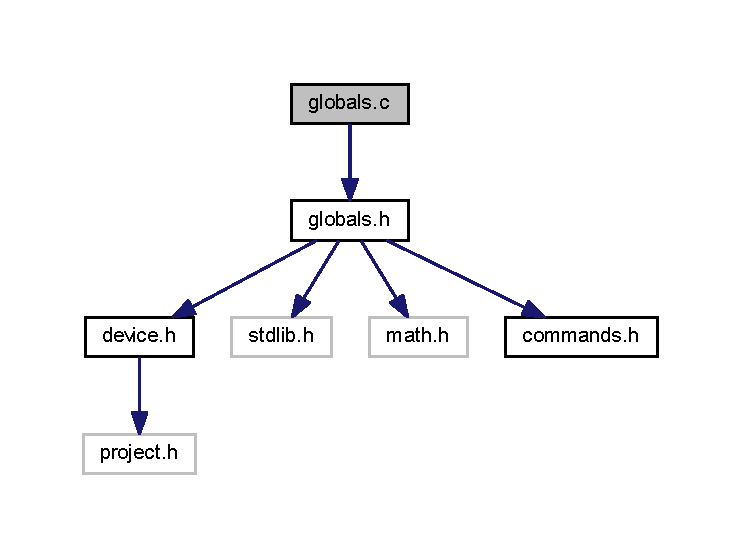
\includegraphics[width=350pt]{globals_8c__incl}
\end{center}
\end{figure}
\subsection*{Variables}
\begin{DoxyCompactItemize}
\item 
\mbox{\label{globals_8c_a158d26b6d15050b37d8039881d75e0dc}} 
struct \textbf{ st\+\_\+ref} g\+\_\+ref g\+\_\+ref\+New {\bfseries g\+\_\+ref\+Old}
\item 
\mbox{\label{globals_8c_a47c3980e6bddec492ca4315e36602ba0}} 
struct \textbf{ st\+\_\+meas} g\+\_\+meas {\bfseries g\+\_\+meas\+Old}
\item 
\mbox{\label{globals_8c_aa963ce8fafc11e104eb7ee22982d0345}} 
struct \textbf{ st\+\_\+data} {\bfseries g\+\_\+rx}
\item 
\mbox{\label{globals_8c_a44c3cbd8e234e0816f0334e29646a800}} 
struct \textbf{ st\+\_\+mem} g\+\_\+mem {\bfseries c\+\_\+mem}
\item 
\mbox{\label{globals_8c_ad47cd0e4d0fcf5739a88e52e949a8084}} 
uint32 {\bfseries timer\+\_\+value}
\item 
\mbox{\label{globals_8c_a9bab7f1b1cf2ba38d5968eee42644c32}} 
uint32 {\bfseries timer\+\_\+value0}
\item 
\mbox{\label{globals_8c_a53a494e9edc739a4f7c884778d1a93b1}} 
int32 {\bfseries dev\+\_\+tension}
\item 
\mbox{\label{globals_8c_a21f4f67e4203dea0b9956589eaa6cef3}} 
uint8 {\bfseries dev\+\_\+pwm\+\_\+limit}
\item 
\mbox{\label{globals_8c_afa36d7a54495dfdb796684539bf041a5}} 
uint8 {\bfseries calibration\+\_\+flag}
\item 
\mbox{\label{globals_8c_aa89a782cfe75ce7970236babd308fe69}} 
C\+Y\+B\+IT {\bfseries reset\+\_\+last\+\_\+value\+\_\+flag}
\item 
\mbox{\label{globals_8c_ac42fa606610c2600210d9b7b2c1d0882}} 
C\+Y\+B\+IT {\bfseries tension\+\_\+valid}
\item 
\mbox{\label{globals_8c_a1e6fda88dfdabc63859f8907eb702920}} 
C\+Y\+B\+IT {\bfseries interrupt\+\_\+flag}
\item 
\mbox{\label{globals_8c_a156a860c465529ff2f515725ab816a58}} 
C\+Y\+B\+IT {\bfseries watchdog\+\_\+flag}
\item 
\mbox{\label{globals_8c_ae87ec724f062d03e4f26473585e6a39f}} 
int16 {\bfseries A\+D\+C\+\_\+buf} [5]
\item 
\mbox{\label{globals_8c_adbb99439f0bdc2e7469e015d16b4d2c2}} 
uint16 {\bfseries pulse\+\_\+counter}
\item 
\mbox{\label{globals_8c_a9a9efe39376a01c0991cedc1a01c0540}} 
C\+Y\+B\+IT {\bfseries motor\+\_\+pulse\+\_\+started} = F\+A\+L\+SE
\item 
\mbox{\label{globals_8c_a0303b07a375125f93a5c178014ae0c6f}} 
float {\bfseries pulse\+\_\+counter\+\_\+float}
\end{DoxyCompactItemize}


\subsection{Detailed Description}
Global variables. 

\begin{DoxyDate}{Date}
October 01, 2017 
\end{DoxyDate}
\begin{DoxyAuthor}{Author}
{\itshape Centro \char`\"{}\+E.\+Piaggio\char`\"{}} 
\end{DoxyAuthor}
\begin{DoxyCopyright}{Copyright}
(C) 2012-\/2016 qbrobotics. All rights reserved. 

(C) 2017 Centro \char`\"{}\+E.\+Piaggio\char`\"{}. All rights reserved. 
\end{DoxyCopyright}

\section{globals.\+h File Reference}
\label{globals_8h}\index{globals.\+h@{globals.\+h}}


Global definitions and macros are set in this file.  


{\ttfamily \#include $<$device.\+h$>$}\newline
{\ttfamily \#include \char`\"{}stdlib.\+h\char`\"{}}\newline
{\ttfamily \#include \char`\"{}math.\+h\char`\"{}}\newline
{\ttfamily \#include \char`\"{}commands.\+h\char`\"{}}\newline
Include dependency graph for globals.\+h\+:
\nopagebreak
\begin{figure}[H]
\begin{center}
\leavevmode
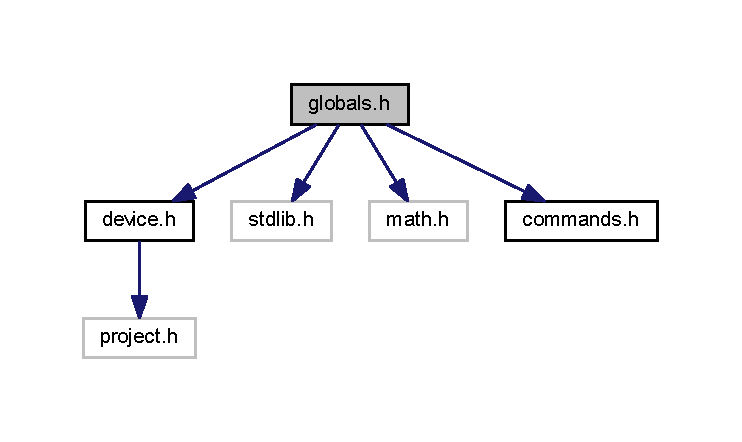
\includegraphics[width=350pt]{globals_8h__incl}
\end{center}
\end{figure}
This graph shows which files directly or indirectly include this file\+:
\nopagebreak
\begin{figure}[H]
\begin{center}
\leavevmode
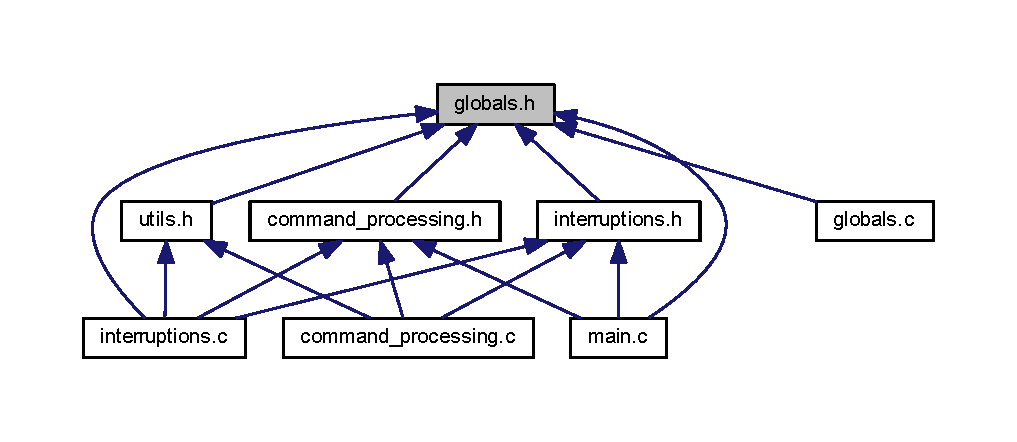
\includegraphics[width=350pt]{globals_8h__dep__incl}
\end{center}
\end{figure}
\subsection*{Data Structures}
\begin{DoxyCompactItemize}
\item 
struct \textbf{ st\+\_\+ref}
\item 
struct \textbf{ st\+\_\+meas}
\item 
struct \textbf{ st\+\_\+data}
\item 
struct \textbf{ st\+\_\+mem}
\end{DoxyCompactItemize}
\subsection*{Macros}
\begin{DoxyCompactItemize}
\item 
\mbox{\label{globals_8h_a1c6d5de492ac61ad29aec7aa9a436bbf}} 
\#define {\bfseries V\+E\+R\+S\+I\+ON}~\char`\"{}W-\/F\+YD M\+OD v6.\+1.\+0\char`\"{}
\item 
\mbox{\label{globals_8h_a39ac50737c1ee7d5b723b2597fdf6f26}} 
\#define {\bfseries N\+U\+M\+\_\+\+O\+F\+\_\+\+M\+O\+T\+O\+RS}~2
\item 
\mbox{\label{globals_8h_af48a6b6fcdc5f5019fb108d03b07a727}} 
\#define {\bfseries N\+U\+M\+\_\+\+O\+F\+\_\+\+S\+E\+N\+S\+O\+RS}~2
\item 
\mbox{\label{globals_8h_a181be7cbd0b2da8e8bb809e6313bd67f}} 
\#define {\bfseries N\+U\+M\+\_\+\+O\+F\+\_\+\+A\+N\+A\+L\+O\+G\+\_\+\+I\+N\+P\+U\+TS}~5
\item 
\mbox{\label{globals_8h_aab4f4a0ece20c4bc27152bd72926d89c}} 
\#define {\bfseries N\+U\+M\+\_\+\+O\+F\+\_\+\+P\+A\+R\+A\+MS}~14
\item 
\mbox{\label{globals_8h_aafe0521fa22763b7afc50e12d31b450d}} 
\#define {\bfseries P\+W\+M\+\_\+\+M\+A\+X\+\_\+\+V\+A\+L\+UE}~100
\item 
\mbox{\label{globals_8h_ada72214f9e15f255cad72a749211b3df}} 
\#define {\bfseries P\+W\+M\+\_\+\+D\+E\+AD}~0
\item 
\mbox{\label{globals_8h_ad252b8b0421e545cce8ba0548a6ca4ed}} 
\#define {\bfseries P\+O\+S\+\_\+\+I\+N\+T\+E\+G\+R\+A\+L\+\_\+\+S\+A\+T\+\_\+\+L\+I\+M\+IT}~100000
\item 
\mbox{\label{globals_8h_a94ec4e208ccec9fc13d0f57094f6de35}} 
\#define {\bfseries C\+U\+R\+R\+\_\+\+I\+N\+T\+E\+G\+R\+A\+L\+\_\+\+S\+A\+T\+\_\+\+L\+I\+M\+IT}~100000
\item 
\mbox{\label{globals_8h_aff0004301ad937f09b58d17ff3f8c9b3}} 
\#define {\bfseries C\+A\+L\+I\+B\+\_\+\+C\+U\+R\+R\+E\+NT}~1000
\item 
\mbox{\label{globals_8h_ae0001cc59fb1ba0290c6ef8c2c5692d7}} 
\#define {\bfseries D\+E\+F\+A\+U\+L\+T\+\_\+\+C\+U\+R\+R\+E\+N\+T\+\_\+\+L\+I\+M\+IT}~1500
\item 
\mbox{\label{globals_8h_a80db2dce057c92400a7fb1678bc0b0a8}} 
\#define {\bfseries C\+A\+L\+I\+B\+R\+A\+T\+I\+O\+N\+\_\+\+D\+IV}~100
\item 
\mbox{\label{globals_8h_a14df76a41da04070ee775565e8d67e81}} 
\#define {\bfseries D\+I\+V\+\_\+\+I\+N\+I\+T\+\_\+\+V\+A\+L\+UE}~1
\item 
\mbox{\label{globals_8h_abf6c9afec04b86961e177e0646401ace}} 
\#define {\bfseries D\+M\+A\+\_\+\+B\+Y\+T\+E\+S\+\_\+\+P\+E\+R\+\_\+\+B\+U\+R\+ST}~2
\item 
\mbox{\label{globals_8h_ab4613f8bee68bc68fa6fe94a3ae6d568}} 
\#define {\bfseries D\+M\+A\+\_\+\+R\+E\+Q\+U\+E\+S\+T\+\_\+\+P\+E\+R\+\_\+\+B\+U\+R\+ST}~1
\item 
\mbox{\label{globals_8h_a3cc2eedb40809a1f15ad841c8abbcebf}} 
\#define {\bfseries D\+M\+A\+\_\+\+S\+R\+C\+\_\+\+B\+A\+SE}~(C\+Y\+D\+E\+V\+\_\+\+P\+E\+R\+I\+P\+H\+\_\+\+B\+A\+SE)
\item 
\mbox{\label{globals_8h_aa54e301f446a66cbf8c943d920c8e967}} 
\#define {\bfseries D\+M\+A\+\_\+\+D\+S\+T\+\_\+\+B\+A\+SE}~(C\+Y\+D\+E\+V\+\_\+\+S\+R\+A\+M\+\_\+\+B\+A\+SE)
\item 
\mbox{\label{globals_8h_aea55597952638136c7c929b238904c82}} 
\#define {\bfseries W\+A\+I\+T\+\_\+\+S\+T\+A\+RT}~0
\item 
\mbox{\label{globals_8h_a6a6a0bb02e515a094c3e7ea1bcb66fcc}} 
\#define {\bfseries W\+A\+I\+T\+\_\+\+ID}~1
\item 
\mbox{\label{globals_8h_a235d2d0eac7e9af190ebafb84df37fd9}} 
\#define {\bfseries W\+A\+I\+T\+\_\+\+L\+E\+N\+G\+TH}~2
\item 
\mbox{\label{globals_8h_a3b4d8a5e259fa47a909adefcda3bfb80}} 
\#define {\bfseries R\+E\+C\+E\+I\+VE}~3
\item 
\mbox{\label{globals_8h_abf4aedd34d31b63b63061c975d872580}} 
\#define {\bfseries U\+N\+L\+O\+AD}~4
\item 
\mbox{\label{globals_8h_aa93f0eb578d23995850d61f7d61c55c1}} 
\#define {\bfseries F\+A\+L\+SE}~0
\item 
\mbox{\label{globals_8h_aa8cecfc5c5c054d2875c03e77b7be15d}} 
\#define {\bfseries T\+R\+UE}~1
\item 
\mbox{\label{globals_8h_a0f5a7e2ead9cd507bf8fc9a6f785f012}} 
\#define {\bfseries D\+E\+F\+A\+U\+L\+T\+\_\+\+E\+E\+P\+R\+O\+M\+\_\+\+D\+I\+S\+P\+L\+A\+C\+E\+M\+E\+NT}~8
\item 
\mbox{\label{globals_8h_a887dbd571d7f138cbe0e994e3fcc661b}} 
\#define {\bfseries M\+A\+X\+\_\+\+W\+A\+T\+C\+H\+D\+O\+G\+\_\+\+T\+I\+M\+ER}~250
\item 
\mbox{\label{globals_8h_a7e2e5b1bc045884a431b736d1013f596}} 
\#define {\bfseries D\+E\+F\+A\+U\+L\+T\+\_\+\+M\+A\+X\+\_\+\+F\+O\+R\+C\+E\+\_\+\+P\+U\+L\+SE}~1900
\item 
\mbox{\label{globals_8h_a1ca2fe6e680bc3f719ae07077b880784}} 
\#define {\bfseries D\+E\+F\+A\+U\+L\+T\+\_\+\+M\+I\+N\+\_\+\+F\+O\+R\+C\+E\+\_\+\+P\+U\+L\+SE}~1350
\item 
\mbox{\label{globals_8h_a88e979262de6afe15c6a99b6c9eee91a}} 
\#define {\bfseries M\+A\+X\+\_\+\+F\+O\+R\+CE}~3520
\item 
\mbox{\label{globals_8h_a786cfa1cc7ee1aa11cceecde022e4db2}} 
\#define {\bfseries M\+I\+N\+\_\+\+F\+O\+R\+CE}~-\/1583
\end{DoxyCompactItemize}
\subsection*{Enumerations}
\begin{DoxyCompactItemize}
\item 
\mbox{\label{globals_8h_a97a989322df9dca90b38ef77610b8301}} 
enum {\bfseries calibration\+\_\+status} \{ \newline
{\bfseries S\+T\+OP} = 0, 
{\bfseries S\+T\+A\+RT} = 1, 
{\bfseries C\+O\+N\+T\+I\+N\+U\+E\+\_\+1} = 2, 
{\bfseries C\+O\+N\+T\+I\+N\+U\+E\+\_\+2} = 3, 
\newline
{\bfseries P\+A\+U\+S\+E\+\_\+1} = 4, 
{\bfseries P\+A\+U\+S\+E\+\_\+2} = 5
 \}
\end{DoxyCompactItemize}
\subsection*{Variables}
\begin{DoxyCompactItemize}
\item 
\mbox{\label{globals_8h_a158d26b6d15050b37d8039881d75e0dc}} 
struct \textbf{ st\+\_\+ref} g\+\_\+ref g\+\_\+ref\+New {\bfseries g\+\_\+ref\+Old}
\item 
\mbox{\label{globals_8h_a47c3980e6bddec492ca4315e36602ba0}} 
struct \textbf{ st\+\_\+meas} g\+\_\+meas {\bfseries g\+\_\+meas\+Old}
\item 
\mbox{\label{globals_8h_aa963ce8fafc11e104eb7ee22982d0345}} 
struct \textbf{ st\+\_\+data} {\bfseries g\+\_\+rx}
\item 
\mbox{\label{globals_8h_a44c3cbd8e234e0816f0334e29646a800}} 
struct \textbf{ st\+\_\+mem} g\+\_\+mem {\bfseries c\+\_\+mem}
\item 
\mbox{\label{globals_8h_ad47cd0e4d0fcf5739a88e52e949a8084}} 
uint32 {\bfseries timer\+\_\+value}
\item 
\mbox{\label{globals_8h_a9bab7f1b1cf2ba38d5968eee42644c32}} 
uint32 {\bfseries timer\+\_\+value0}
\item 
\mbox{\label{globals_8h_a53a494e9edc739a4f7c884778d1a93b1}} 
int32 {\bfseries dev\+\_\+tension}
\item 
\mbox{\label{globals_8h_a21f4f67e4203dea0b9956589eaa6cef3}} 
uint8 {\bfseries dev\+\_\+pwm\+\_\+limit}
\item 
\mbox{\label{globals_8h_afa36d7a54495dfdb796684539bf041a5}} 
uint8 {\bfseries calibration\+\_\+flag}
\item 
\mbox{\label{globals_8h_aa89a782cfe75ce7970236babd308fe69}} 
C\+Y\+B\+IT {\bfseries reset\+\_\+last\+\_\+value\+\_\+flag}
\item 
\mbox{\label{globals_8h_ac42fa606610c2600210d9b7b2c1d0882}} 
C\+Y\+B\+IT {\bfseries tension\+\_\+valid}
\item 
\mbox{\label{globals_8h_a1e6fda88dfdabc63859f8907eb702920}} 
C\+Y\+B\+IT {\bfseries interrupt\+\_\+flag}
\item 
\mbox{\label{globals_8h_a156a860c465529ff2f515725ab816a58}} 
C\+Y\+B\+IT {\bfseries watchdog\+\_\+flag}
\item 
\mbox{\label{globals_8h_ae87ec724f062d03e4f26473585e6a39f}} 
int16 {\bfseries A\+D\+C\+\_\+buf} [5]
\item 
\mbox{\label{globals_8h_adbb99439f0bdc2e7469e015d16b4d2c2}} 
uint16 {\bfseries pulse\+\_\+counter}
\item 
\mbox{\label{globals_8h_a0303b07a375125f93a5c178014ae0c6f}} 
float {\bfseries pulse\+\_\+counter\+\_\+float}
\item 
\mbox{\label{globals_8h_a9a9efe39376a01c0991cedc1a01c0540}} 
C\+Y\+B\+IT {\bfseries motor\+\_\+pulse\+\_\+started}
\end{DoxyCompactItemize}


\subsection{Detailed Description}
Global definitions and macros are set in this file. 

\begin{DoxyDate}{Date}
October 01, 2017 
\end{DoxyDate}
\begin{DoxyAuthor}{Author}
{\itshape Centro \char`\"{}\+E.\+Piaggio\char`\"{}} 
\end{DoxyAuthor}
\begin{DoxyCopyright}{Copyright}
(C) 2012-\/2016 qbrobotics. All rights reserved. 

(C) 2017 Centro \char`\"{}\+E.\+Piaggio\char`\"{}. All rights reserved. 
\end{DoxyCopyright}

\section{interruptions.\+c File Reference}
\label{interruptions_8c}\index{interruptions.\+c@{interruptions.\+c}}


Interruption functions are in this file.  


{\ttfamily \#include $<$interruptions.\+h$>$}\newline
{\ttfamily \#include $<$command\+\_\+processing.\+h$>$}\newline
{\ttfamily \#include \char`\"{}globals.\+h\char`\"{}}\newline
{\ttfamily \#include \char`\"{}utils.\+h\char`\"{}}\newline
Include dependency graph for interruptions.\+c\+:
\nopagebreak
\begin{figure}[H]
\begin{center}
\leavevmode
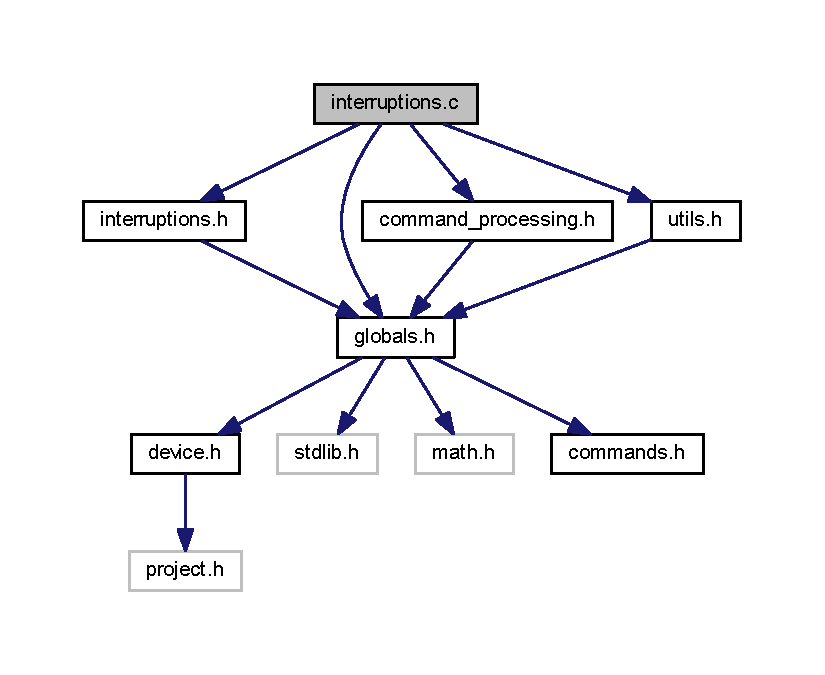
\includegraphics[width=350pt]{interruptions_8c__incl}
\end{center}
\end{figure}
\subsection*{Functions}
\begin{DoxyCompactItemize}
\item 
\mbox{\label{interruptions_8c_aba74df0c62c62434ebccf8124c5d5fef}} 
{\bfseries C\+Y\+\_\+\+I\+SR} (I\+S\+R\+\_\+\+W\+A\+T\+C\+H\+D\+O\+G\+\_\+\+Handler)
\item 
\mbox{\label{interruptions_8c_a7692d8c3185943c5bdfaa6de0a172ad3}} 
{\bfseries C\+Y\+\_\+\+I\+SR} (I\+S\+R\+\_\+\+R\+S485\+\_\+\+R\+X\+\_\+\+Ex\+Interrupt)
\item 
\mbox{\label{interruptions_8c_a9790811526002d99b25a814afd02cbae}} 
void {\bfseries interrupt\+\_\+manager} ()
\item 
\mbox{\label{interruptions_8c_a39df971c4e9f194be50c54dfd7aeabfe}} 
void {\bfseries function\+\_\+scheduler} (void)
\item 
\mbox{\label{interruptions_8c_a717216ab689fc8b8ea3fb8795a816a2b}} 
void {\bfseries motor\+\_\+control} (const uint8 idx)
\item 
\mbox{\label{interruptions_8c_a00a8d34962a63161405e5d7785b9625e}} 
void {\bfseries analog\+\_\+read\+\_\+end} ()
\item 
\mbox{\label{interruptions_8c_ac8679c9d627ace495295abdacbc7dcf2}} 
void {\bfseries encoder\+\_\+reading} (const uint8 idx, const uint8 flag)
\item 
\mbox{\label{interruptions_8c_a6d9dc88d64cd1f74a30fd0e404a3bb31}} 
void {\bfseries calibration} ()
\item 
\mbox{\label{interruptions_8c_ab7b287cf5df2ea548297b951be2f20d4}} 
void {\bfseries pwm\+\_\+limit\+\_\+search} ()
\item 
\mbox{\label{interruptions_8c_a454a1d47ea0044672f38fe2199518846}} 
void {\bfseries set\+\_\+servo} (int16 duty)
\item 
\mbox{\label{interruptions_8c_a820fef0be6eb876b1ab318e1dedd568c}} 
void {\bfseries get\+\_\+servo} ()
\end{DoxyCompactItemize}
\subsection*{Variables}
\begin{DoxyCompactItemize}
\item 
C\+Y\+C\+O\+DE uint8 {\bfseries pwm\+\_\+preload\+\_\+values} [29]
\item 
\mbox{\label{interruptions_8c_a4234b71c84e0fb74d3ad698276b90f6e}} 
C\+Y\+C\+O\+DE uint8 {\bfseries hitech\+\_\+pwm\+\_\+preload\+\_\+values} [36]
\item 
\mbox{\label{interruptions_8c_a6dc1a7b985a28e3db77fad72bfbc0b46}} 
C\+Y\+C\+O\+DE uint8 {\bfseries hitech\+\_\+pwm\+\_\+preload\+\_\+values\+\_\+6v} [32]
\end{DoxyCompactItemize}


\subsection{Detailed Description}
Interruption functions are in this file. 

\begin{DoxyDate}{Date}
October 01, 2017 
\end{DoxyDate}
\begin{DoxyAuthor}{Author}
{\itshape Centro \char`\"{}\+E.\+Piaggio\char`\"{}} 
\end{DoxyAuthor}
\begin{DoxyCopyright}{Copyright}
(C) 2012-\/2016 qbrobotics. All rights reserved. 

(C) 2017 Centro \char`\"{}\+E.\+Piaggio\char`\"{}. All rights reserved. 
\end{DoxyCopyright}


\subsection{Variable Documentation}
\mbox{\label{interruptions_8c_a82beecb0593499956eb3ee6fdf734a76}} 
\index{interruptions.\+c@{interruptions.\+c}!pwm\+\_\+preload\+\_\+values@{pwm\+\_\+preload\+\_\+values}}
\index{pwm\+\_\+preload\+\_\+values@{pwm\+\_\+preload\+\_\+values}!interruptions.\+c@{interruptions.\+c}}
\subsubsection{pwm\+\_\+preload\+\_\+values}
{\footnotesize\ttfamily C\+Y\+C\+O\+DE uint8 pwm\+\_\+preload\+\_\+values[29]}

{\bfseries Initial value\+:}
\begin{DoxyCode}
= \{100,    
                                             100,
                                             100,
                                              76,
                                              74,
                                              72,    
                                              70,
                                              68,
                                              67,
                                              65,
                                              64,    
                                              63,
                                              62,
                                              61,
                                              60,
                                              59,    
                                              58,
                                              57,
                                              56,
                                              56,
                                              55,    
                                              54,
                                              54,
                                              53,
                                              52,
                                              52,    
                                              52,
                                              51,
                                              51\}
\end{DoxyCode}

\section{interruptions.\+h File Reference}
\label{interruptions_8h}\index{interruptions.\+h@{interruptions.\+h}}


Interruptions header file.  


{\ttfamily \#include $<$globals.\+h$>$}\newline
Include dependency graph for interruptions.\+h\+:
\nopagebreak
\begin{figure}[H]
\begin{center}
\leavevmode
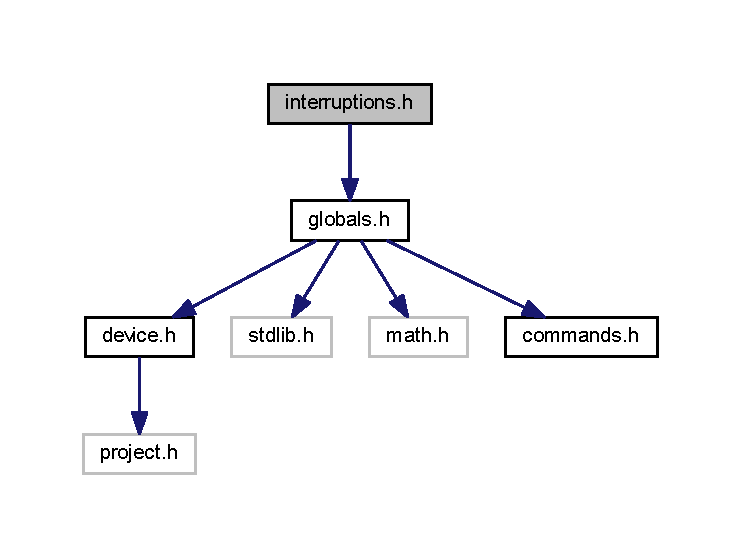
\includegraphics[width=350pt]{interruptions_8h__incl}
\end{center}
\end{figure}
This graph shows which files directly or indirectly include this file\+:
\nopagebreak
\begin{figure}[H]
\begin{center}
\leavevmode
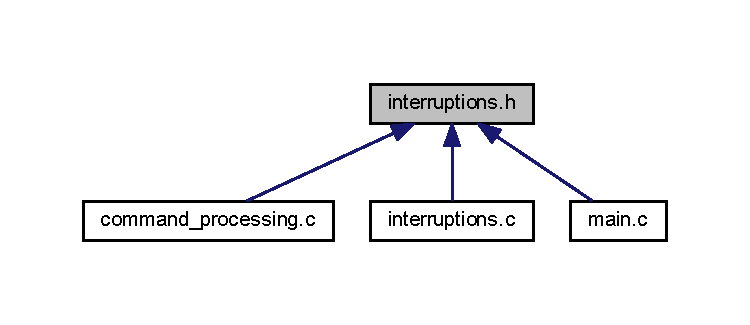
\includegraphics[width=350pt]{interruptions_8h__dep__incl}
\end{center}
\end{figure}
\subsection*{Functions}
\begin{DoxyCompactItemize}
\item 
\mbox{\label{interruptions_8h_a7e24af8c83537b0441877bf0f00dd30a}} 
{\bfseries C\+Y\+\_\+\+I\+S\+R\+\_\+\+P\+R\+O\+TO} (I\+S\+R\+\_\+\+R\+S485\+\_\+\+R\+X\+\_\+\+Ex\+Interrupt)
\item 
\mbox{\label{interruptions_8h_a212cae8995d67d612c236fb54a4d29dc}} 
{\bfseries C\+Y\+\_\+\+I\+S\+R\+\_\+\+P\+R\+O\+TO} (I\+S\+R\+\_\+\+W\+A\+T\+C\+H\+D\+O\+G\+\_\+\+Handler)
\item 
\mbox{\label{interruptions_8h_a39df971c4e9f194be50c54dfd7aeabfe}} 
void {\bfseries function\+\_\+scheduler} (void)
\item 
\mbox{\label{interruptions_8h_a2d58475fb61b7d077e6c34ccf0499198}} 
void {\bfseries encoder\+\_\+reading} (const uint8, const uint8)
\item 
\mbox{\label{interruptions_8h_a94830a771fd71aa5b49ce0b08207985b}} 
void {\bfseries motor\+\_\+control} (const uint8)
\item 
\mbox{\label{interruptions_8h_a00a8d34962a63161405e5d7785b9625e}} 
void {\bfseries analog\+\_\+read\+\_\+end} ()
\item 
\mbox{\label{interruptions_8h_a0b6a0b24c6bd8af032a6778166201f7e}} 
void {\bfseries calibration} (void)
\item 
\mbox{\label{interruptions_8h_ab7b287cf5df2ea548297b951be2f20d4}} 
void {\bfseries pwm\+\_\+limit\+\_\+search} ()
\item 
\mbox{\label{interruptions_8h_a9790811526002d99b25a814afd02cbae}} 
void {\bfseries interrupt\+\_\+manager} ()
\item 
\mbox{\label{interruptions_8h_a4b6ca03597ea8b3ed64bec9806f93549}} 
void {\bfseries set\+\_\+servo} (int16)
\item 
\mbox{\label{interruptions_8h_a820fef0be6eb876b1ab318e1dedd568c}} 
void {\bfseries get\+\_\+servo} ()
\end{DoxyCompactItemize}


\subsection{Detailed Description}
Interruptions header file. 

\begin{DoxyDate}{Date}
October 01, 2017 
\end{DoxyDate}
\begin{DoxyAuthor}{Author}
{\itshape Centro \char`\"{}\+E.\+Piaggio\char`\"{}} 
\end{DoxyAuthor}
\begin{DoxyCopyright}{Copyright}
(C) 2012-\/2016 qbrobotics. All rights reserved. 

(C) 2017 Centro \char`\"{}\+E.\+Piaggio\char`\"{}. All rights reserved. 
\end{DoxyCopyright}

\section{main.\+c File Reference}
\label{main_8c}\index{main.\+c@{main.\+c}}


Firmware main file.  


{\ttfamily \#include $<$device.\+h$>$}\newline
{\ttfamily \#include $<$globals.\+h$>$}\newline
{\ttfamily \#include $<$interruptions.\+h$>$}\newline
{\ttfamily \#include $<$command\+\_\+processing.\+h$>$}\newline
Include dependency graph for main.\+c\+:
\nopagebreak
\begin{figure}[H]
\begin{center}
\leavevmode
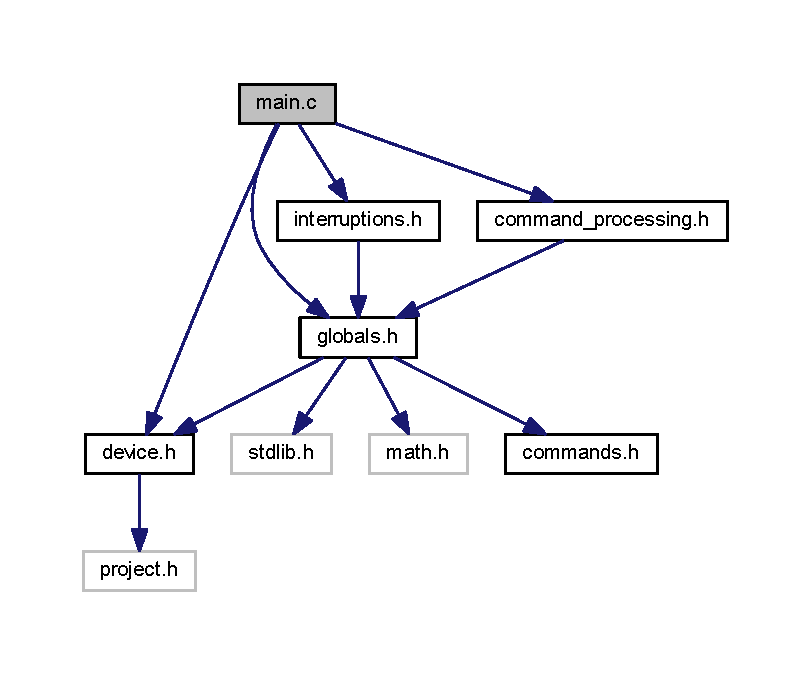
\includegraphics[width=350pt]{main_8c__incl}
\end{center}
\end{figure}
\subsection*{Functions}
\begin{DoxyCompactItemize}
\item 
\mbox{\label{main_8c_ae66f6b31b5ad750f1fe042a706a4e3d4}} 
int {\bfseries main} ()
\end{DoxyCompactItemize}


\subsection{Detailed Description}
Firmware main file. 

\begin{DoxyDate}{Date}
October 01, 2017 
\end{DoxyDate}
\begin{DoxyAuthor}{Author}
{\itshape Centro \char`\"{}\+E.\+Piaggio\char`\"{}} 
\end{DoxyAuthor}
\begin{DoxyCopyright}{Copyright}
(C) 2012-\/2016 qbrobotics. All rights reserved. 

(C) 2017 Centro \char`\"{}\+E.\+Piaggio\char`\"{}. All rights reserved. 
\end{DoxyCopyright}

\section{utils.\+h File Reference}
\label{utils_8h}\index{utils.\+h@{utils.\+h}}


Definition of utility functions.  


{\ttfamily \#include $<$globals.\+h$>$}\newline
Include dependency graph for utils.\+h\+:
\nopagebreak
\begin{figure}[H]
\begin{center}
\leavevmode
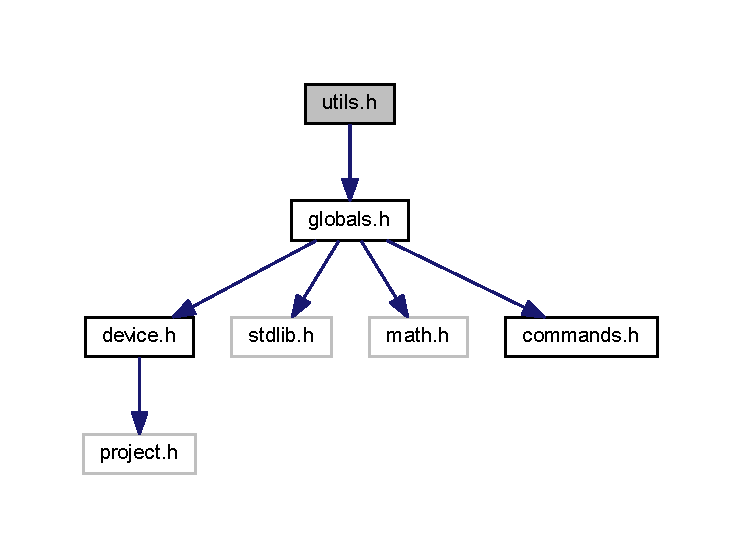
\includegraphics[width=350pt]{utils_8h__incl}
\end{center}
\end{figure}
This graph shows which files directly or indirectly include this file\+:
\nopagebreak
\begin{figure}[H]
\begin{center}
\leavevmode
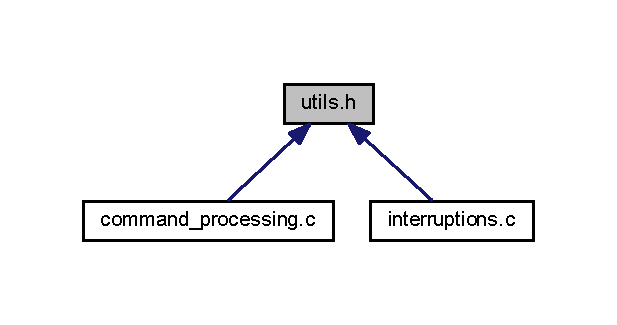
\includegraphics[width=296pt]{utils_8h__dep__incl}
\end{center}
\end{figure}
\subsection*{Macros}
\begin{DoxyCompactItemize}
\item 
\mbox{\label{utils_8h_a8c7db0cde6d591a5abad279ba92ef021}} 
\#define {\bfseries S\+I\+GN}(A)~(((A) $>$ 0) ? (1) \+: ((((A) $<$ 0) ? (-\/1) \+: (0))))
\end{DoxyCompactItemize}
\subsection*{Functions}
\begin{DoxyCompactItemize}
\item 
\mbox{\label{utils_8h_a3588bc1aa14c6ea245387dda7eb7ffbe}} 
int32 {\bfseries filter\+\_\+i1} (int32 value)
\item 
\mbox{\label{utils_8h_ac9c746215432427ee4e8d7dbb84b1c1a}} 
int32 {\bfseries filter\+\_\+i2} (int32 value)
\item 
\mbox{\label{utils_8h_ad378840ee71c2d41d2d4f1a84465c7f3}} 
int32 {\bfseries filter\+\_\+vel\+\_\+1} (int32 value)
\item 
\mbox{\label{utils_8h_abda54d76e676bb1cb27b5577bd0fe099}} 
int32 {\bfseries filter\+\_\+vel\+\_\+2} (int32 value)
\item 
\mbox{\label{utils_8h_a70430ee90ed28e4c9fca0c4ca3d6583e}} 
int32 {\bfseries filter\+\_\+vel\+\_\+3} (int32 value)
\item 
\mbox{\label{utils_8h_a6205a6e88f72f4cc321a7d8abca23e26}} 
uint8 {\bfseries L\+C\+R\+Checksum} (uint8 $\ast$data\+\_\+array, uint8 data\+\_\+length)
\item 
\mbox{\label{utils_8h_a8f6aff189d5fbbb0be1fdd13e0e720c0}} 
C\+Y\+B\+IT {\bfseries check\+\_\+enc\+\_\+data} (const uint32 $\ast$)
\end{DoxyCompactItemize}


\subsection{Detailed Description}
Definition of utility functions. 

Declaration of utility functions.

\begin{DoxyDate}{Date}
October 01, 2017 
\end{DoxyDate}
\begin{DoxyAuthor}{Author}
{\itshape Centro \char`\"{}\+E.\+Piaggio\char`\"{}} 
\end{DoxyAuthor}
\begin{DoxyCopyright}{Copyright}
(C) 2012-\/2016 qbrobotics. All rights reserved. 

(C) 2017 Centro \char`\"{}\+E.\+Piaggio\char`\"{}. All rights reserved. 
\end{DoxyCopyright}

%--- End generated contents ---

% Index
\backmatter
\newpage
\phantomsection
\clearemptydoublepage
\addcontentsline{toc}{chapter}{Index}
\printindex

\end{document}
